\documentclass[12pt]{article}

% ------------------------------------------------------------------
% CORE DOCUMENT SETUP & FONT (XeLaTeX with Libertinus)
% ------------------------------------------------------------------
\usepackage[quiet]{fontspec}
\usepackage{libertinus-otf}
\usepackage[stretch=10,shrink=10]{microtype}
\usepackage[margin=1in]{geometry} % Standard margins
\usepackage{adjustbox}

% ------------------------------------------------------------------
% LAYOUT & SPACING
% ------------------------------------------------------------------
\usepackage{setspace} % For line spacing (e.g., \onehalfspacing)
\usepackage{fancyhdr} % For customizing headers/footers
\usepackage{placeins} % Provides \FloatBarrier to stop floats from moving
\usepackage{pdflscape} % For landscape pages
\usepackage{framed} % For framed boxes/environments
\usepackage[all]{nowidow} % Prevents widows and orphans


% ------------------------------------------------------------------
% HYPERLINKS, REFERENCES, & DOCUMENT STRUCTURE
% ------------------------------------------------------------------
\usepackage{varioref}
\usepackage[title,titletoc,page]{appendix} % Handles appendix structure
\usepackage{minitoc} % For sectional tables of contents
\usepackage{tocloft} % For customizing TOC, list of tables/figures
\usepackage{titletoc} % For local/partial TOCs

% ------------------------------------------------------------------
% TABLES, FIGURES, & CAPTIONS (Grouping Redundant Packages)
% ------------------------------------------------------------------
% NOTE: Removed duplicate loading of caption/subcaption/threeparttable
\usepackage{graphicx}
 % For including figures
\usepackage{subcaption} % Handles subfigures and subtables (modern standard)
\usepackage{caption} % Customizes captions (must be loaded before subcaption in some cases)
\usepackage{booktabs} % Best practice for professional table rules (\toprule, \midrule)
\usepackage[table]{xcolor} % For table cell coloring (\cellcolor)
\usepackage{dcolumn} % For aligning numbers on decimal point in stargazer tables
\usepackage{threeparttable} % For aligning notes under tables (best practice for academic notes)
\usepackage{siunitx} % For formatting units and aligning numbers by decimal point (must have)
\usepackage{multirow} % For cells spanning multiple rows
\usepackage{bigdelim} % For large delimiters in tables (like \rdelim)
\usepackage{xltabular} % Combines xtabular (multi-page tables) and tabularx (fixed width columns)

% ------------------------------------------------------------------
% MISCELLANEOUS UTILITIES
% ------------------------------------------------------------------
\usepackage{natbib} % Citation package (assuming you use BibTeX/BibLaTeX)
\usepackage{enumitem} % For customizing lists (spacing, labels, etc.)
\usepackage{epigraph} % For block quotes
\usepackage{pifont} % For Zapf Dingbats symbols (cmark/xmark)
\newcommand{\xmark}{\ding{53}}%
\newcommand{\cmark}{\ding{51}}%
\AtBeginDocument{\renewcommand{\checkmark}{\text{\ding{51}}}}%
\usepackage{tikz} % For drawing graphics
\usepackage{comment} % For commenting out large blocks of text

\usetikzlibrary{positioning, calc, arrows, arrows.meta, decorations.markings, decorations.pathmorphing, shapes.misc, matrix, shapes, fit, tikzmark}

\tikzset{
    block/.style = {rectangle, draw, text centered, rounded corners, minimum height=1.5em},
    line/.style = {draw, -latex'},
    snake/.style = {decorate, decoration={snake}},
}

% ------------------------------------------------------------------
% HYPERLINKS (load after other packages, before custom commands)
% ------------------------------------------------------------------
\usepackage{hyperref}
\hypersetup{
    colorlinks=true,
    linkcolor=blue,
    citecolor=black,
    urlcolor=blue
}
\usepackage[all]{hypcap}

% ------------------------------------------------------------------
% MANUAL/CUSTOM COMMANDS (Keep these at the very end)
% ------------------------------------------------------------------
% Make the "Part I" text invisible
\renewcommand \thepart{}
\renewcommand \partname{}

\setlength{\epigraphwidth}{\textwidth}
\renewcommand{\arraystretch}{1.15}
\title{The Limits of Electoral Gender Quotas in Rural Local Bodies}

% Intercepted: Male Gatekeeping and the Limits of Gender Quotas in Rural India
% "Intercepted: Gender Quotas and  Male Gatekeeping  in Rural India


%The Limits of Gender Quotas: Formal Inclusion, Effective Exclusion in Rural India"

%The Limits of Gender Quotas: De Jure Representation and De Facto Gatekeeping in Rural India
%The Limits of Electoral Gender Quotas: Evidence from Rural India
%Formal Inclusion, Effective Exclusion: Gender Quotas and Barriers to Women's Representation in Rural India

%\thanks{The authors gratefully acknowledge The Center for International Studies at the University of Southern California for funding a part of this research. We thank audiences at the 2025 Rebecca B. Morton Conference on Experimental Political Science in New York University, 2025 New Perspectives on the Political Economy of Development Conference at University of Southern California,   PIPE Workshop 2024 in USC Price School of Public Policy, Brown-Harvard South Asia seminar 2024, CIS Comparative Workshop Series (2024 -- 25) in the University of Southern California, Annual Meeting of the American Political Science Association 2024,  PolMeth 2024 poster presentation session, SoCal Pipe at UCLA Fall 2024, CLASS workshop in Gould School of Law. We are grateful to Aidan Milliff, Alexander Coppock, Alyssa Heinze, Amanda Clayton, Amna Salam, Ana Catalano Weeks, Arturas Rozenas, Christian Phillips, Chris Dawes, Claire Adida,  Don Green, Erik Hanson, Evan Lieberman, Feyaad Allie, Gwyneth McClendon, Jason Lyall, Jeff Weaver, Jennifer Piscopo, Jessica Sun, Julia Payson, Luke Sanford, Marcel Fafchamps, Maria Silfa, Par Zetterberg, Pradeep Chhibber, Rebecca Weitz-Shapiro,  Rikhil Bhavnani,  Shikhar Singh,  Thibaud Marcesse,  Tom Pepinsky, and Zuheir Desai for helpful comments. All errors are our responsibility.}
% \usepackage{floatrow}
% \floatsetup[table]{framestyle=,framearound=none,heightadjust=none}
% \floatsetup[figure]{framestyle=,framearound=none,heightadjust=none}

\author{Varun Karekurve-Ramachandra\thanks{Assistant Professor, Department of Political Science and International Relations, University of Southern California, Email: \href{mailto:varun.rama@usc.edu}{varun.rama@usc.edu}} \and Gaurav Sood\thanks{Independent Researcher, Email: \href{mailto:gsood07@gmail.com}{gsood07@gmail.com}}} 

\date{\today}

\newcommand{\rajShortOne}{1.4}
\newcommand{\rajShortOneLow}{-0.4}
\newcommand{\rajShortOneHigh}{3.3}
\newcommand{\rajShortTwo}{-2.8}
\newcommand{\rajShortTwoLow}{-5.1}
\newcommand{\rajShortTwoHigh}{-0.6}
\newcommand{\rajShortThree}{0.4}
\newcommand{\rajShortThreeLow}{-1.8}
\newcommand{\rajShortThreeHigh}{2.7}
\newcommand{\rajFullAlways}{9.4}
\newcommand{\rajFullAlwaysLow}{2.8}
\newcommand{\rajFullAlwaysHigh}{16.0}
\newcommand{\rajFullAlwaysN}{2,671}
\newcommand{\rajFullAlwaysLeftN}{149}
\newcommand{\rajFullAlwaysRightN}{225}
\newcommand{\rajFullAlwaysSharedClusters}{65}
\newcommand{\rajFullExtra}{5.3}
\newcommand{\rajFullExtraLow}{-1.0}
\newcommand{\rajFullExtraHigh}{11.7}
\newcommand{\rajFullExtraN}{2,671}
\newcommand{\rajFullExtraLeftN}{149}
\newcommand{\rajFullExtraRightN}{873}
\newcommand{\rajFullExtraSharedClusters}{88}
\newcommand{\rajRestrictedAlways}{6.7}
\newcommand{\rajRestrictedAlwaysLow}{-3.1}
\newcommand{\rajRestrictedAlwaysHigh}{16.5}
\newcommand{\rajRestrictedAlwaysN}{601}
\newcommand{\rajRestrictedAlwaysLeftN}{58}
\newcommand{\rajRestrictedAlwaysRightN}{77}
\newcommand{\rajRestrictedAlwaysSharedClusters}{31}
\newcommand{\rajRestrictedExtra}{-2.4}
\newcommand{\rajRestrictedExtraLow}{-12.3}
\newcommand{\rajRestrictedExtraHigh}{7.6}
\newcommand{\rajRestrictedExtraN}{601}
\newcommand{\rajRestrictedExtraLeftN}{58}
\newcommand{\rajRestrictedExtraRightN}{153}
\newcommand{\rajRestrictedExtraSharedClusters}{37}
\newcommand{\upShortOne}{2.1}
\newcommand{\upShortOneLow}{1.2}
\newcommand{\upShortOneHigh}{2.9}
\newcommand{\upShortTwo}{1.6}
\newcommand{\upShortTwoLow}{0.7}
\newcommand{\upShortTwoHigh}{2.6}
\newcommand{\upShortThree}{3.6}
\newcommand{\upShortThreeLow}{2.6}
\newcommand{\upShortThreeHigh}{4.5}
\newcommand{\upFullAlways}{7.7}
\newcommand{\upFullAlwaysLow}{4.5}
\newcommand{\upFullAlwaysHigh}{10.9}
\newcommand{\upFullAlwaysN}{19,264}
\newcommand{\upFullAlwaysLeftN}{798}
\newcommand{\upFullAlwaysRightN}{2,916}
\newcommand{\upFullAlwaysSharedClusters}{385}
\newcommand{\upFullExtra}{4.0}
\newcommand{\upFullExtraLow}{0.8}
\newcommand{\upFullExtraHigh}{7.1}
\newcommand{\upFullExtraN}{19,264}
\newcommand{\upFullExtraLeftN}{798}
\newcommand{\upFullExtraRightN}{3,978}
\newcommand{\upFullExtraSharedClusters}{392}
\newcommand{\upRestrictedAlways}{8.4}
\newcommand{\upRestrictedAlwaysLow}{1.2}
\newcommand{\upRestrictedAlwaysHigh}{15.6}
\newcommand{\upRestrictedAlwaysN}{2,952}
\newcommand{\upRestrictedAlwaysLeftN}{149}
\newcommand{\upRestrictedAlwaysRightN}{426}
\newcommand{\upRestrictedAlwaysSharedClusters}{65}
\newcommand{\upRestrictedExtra}{1.4}
\newcommand{\upRestrictedExtraLow}{-5.9}
\newcommand{\upRestrictedExtraHigh}{8.6}
\newcommand{\upRestrictedExtraN}{2,952}
\newcommand{\upRestrictedExtraLeftN}{149}
\newcommand{\upRestrictedExtraRightN}{602}
\newcommand{\upRestrictedExtraSharedClusters}{68}
\newcommand{\shortMdeMin}{1.2}
\newcommand{\shortMdeMax}{3.2}
\newcommand{\longMdeMin}{4.6}
\newcommand{\longMdeMax}{9.2}
\newcommand{\allAgeOpen}{42.8}
\newcommand{\allAgeQuota}{41.2}
\newcommand{\allGraduateOpen}{23.6}
\newcommand{\allGraduateQuota}{12.3}
\newcommand{\allUnemployedOpen}{9.9}
\newcommand{\allUnemployedQuota}{60.9}
\newcommand{\allLogassetsOpen}{12.9}
\newcommand{\allLogassetsQuota}{12.6}
\newcommand{\womenAgeOpen}{42.8}
\newcommand{\womenAgeQuota}{41.2}
\newcommand{\womenGraduateOpen}{11.5}
\newcommand{\womenGraduateQuota}{12.3}
\newcommand{\womenUnemployedOpen}{53.1}
\newcommand{\womenUnemployedQuota}{61.1}
\newcommand{\womenLogassetsOpen}{12.6}
\newcommand{\womenLogassetsQuota}{12.6}

\begin{document}

\maketitle



\begin{abstract}
\noindent We study whether women win unreserved seats at higher rates when those seats were previously reserved. Our data cover over 25,000 local government bodies across four election cycles spanning sixteen years in rural India, where seats are randomly reserved for women. In Rajasthan, prior reservation has small negative or positive effects on women's subsequent electoral success. In Uttar Pradesh, effects are positive but small: 1–4 percentage points on a base of 14–19\%, well below the roughly 18 percentage point effects documented in urban settings. Short-run minimum detectable effects range from \shortMdeMin{} to \shortMdeMax{} percentage points. Three prior reservations versus none are associated with gains of \rajFullAlways{} percentage points in Rajasthan and \upFullAlways{} in UP; restricted-sample estimates are less precise and do not show that these gains disappear. Phone audits covering roughly 1,000 representatives reveal a mechanism: male non-members answered 85\% of answered calls to quota-seat officeholders, and only 9\% of calls reached the elected woman herself, compared with 76\% in open seats. Women elected under quotas are also younger, less educated, and less wealthy than their open-seat counterparts. Quotas achieve \textit{de jure} representation but, where male relatives govern by proxy, do not create the conditions for women to retain power independently.


\vspace{6mm}

\noindent \textbf{Keywords:} Women in Politics, Gender Quotas, India, Local Government

\end{abstract}

\thispagestyle{empty}

\newpage
\FloatBarrier

\pagenumbering{arabic}
\doublespacing

\section{Introduction}

Women's representation in elected office matters for both intrinsic and instrumental reasons. Equal citizenship is difficult to reconcile with decision-making bodies in which half the population is largely absent. The instrumental case is equally strong: India's political reservations for women show that female leaders shift spending toward public goods preferred by women \citep{chattopadhyay2004women}, that exposure to women leaders narrows gender gaps in aspirations by 20--32\% and eliminates gender gaps in educational attainment \citep{beaman2012female}, and that women's political voice strengthens institutional responsiveness, including greater reporting of crimes against women \citep{iyer2012power}. Despite this evidence, women remain sharply underrepresented in elected bodies worldwide. Many countries have adopted electoral quotas in response, betting that temporary mandates will prove self-sustaining: exposure to female leaders shifts voter attitudes, women acquire political skills and networks, and a pipeline of viable candidates emerges that no longer depends on the quota.

We test this expectation in rural India, where a constitutional mandate reserves at least one third of local government leadership positions for women. Using sixteen years of electoral data from over 25,000 Gram Panchayats across four election cycles in Rajasthan and Uttar Pradesh, we ask whether seats previously reserved for women are more likely to elect women once the reservation is lifted.

We find that prior reservation has limited effects on women's subsequent electoral success. In Rajasthan, short-run estimates range from a small negative effect to small positive effects. In Uttar Pradesh, effects are positive but small: 1--4 percentage points on a base of 14--19\%, well below the roughly 18 percentage point effect \citet{bhavnani2009electoral} documented in urban Mumbai. Short-run minimum detectable effects at 80\% power range from \shortMdeMin{} to \shortMdeMax{} percentage points. The cumulative comparisons are larger: three prior reservations versus none are associated with gains of \rajFullAlways{} points in Rajasthan and \upFullAlways{} in UP. Pairwise interaction coefficients alone do not measure these cumulative contrasts.

We document two features of the institutional environment that help explain these results. First, male relatives perform the representative function in the vast majority of quota seats. In a phone audit covering roughly 1,000 Sarpanches in Rajasthan, only 9\% of calls to quota-seat representatives reached the elected officeholder; 85\% were answered by male non-members, including 69\% explicitly recorded as relatives. In open seats, 76\% of calls reached the representative directly. This proxy governance severs the causal chain at its first link: if citizens interact with male relatives rather than the female officeholder, voters cannot update their beliefs about women's leadership, and women in office cannot accumulate the political capital or visibility that would let them or others compete without a quota.

Second, women elected under quotas are less professionalized than open-seat winners. In Rajasthan, quota-seat winners are younger, have 11 percentage points lower graduation rates (12\% vs.\ 24\%), own fewer assets, and are far more likely to report being unemployed (61\% vs.\ 10\%). These gaps may reinforce rather than challenge voter stereotypes about women's political competence, further weakening the exposure channel.

A suggestive piece of evidence on scope conditions comes from extending the phone audit to urban Jaipur, where 31.7\% of calls to quota-seat representatives reached the elected officeholder, compared with 9\% in rural areas. Proxy governance is less prevalent in urban settings, though it remains the norm even there. This gradient is consistent with the gap between our rural results and the large urban effects reported by \citet{bhavnani2009electoral}, and suggests that the conditions under which quotas generate lasting representation---women actually governing, a professionalized female candidate pool, voter exposure to female leadership---are more likely to be met in urban settings where household structures and labor markets differ.

Our contribution is threefold. First, we provide the largest and longest test of whether electoral quotas produce lasting gains in women's representation, covering over 25,000 electoral bodies across sixteen years. Previous studies of lasting electoral effects examined single cities or single transitions \citep{bhavnani2009electoral, clayton2018women}. Our data span two states, four election cycles each, and allow us to compare the effects of single and repeated quota exposure. Second, our phone audit provides direct evidence of male proxy governance at scale, revealing how formal inclusion can coexist with effective exclusion from power \citep{valdini2019inclusion, brule2023actually, meguid2025strategic}. Third, the contrast between our rural results and the large urban effects in \citet{bhavnani2009electoral} helps delineate the scope conditions under which quotas can and cannot generate self-sustaining representation.

The implication is not that quotas are ineffective. Quotas guarantee descriptive representation, and compliance with India's mandate has placed nearly a million women in elected local office. The implication is that quotas alone are insufficient to generate self-sustaining female representation in settings where household-level power structures prevent women from exercising the authority that office confers. Complementary interventions that address proxy governance directly may be necessary for quotas to fulfill their transformative potential.

\section{Theoretical Framework}\label{sec:theory}
For quotas to generate lasting change, they must shift either voter behavior or the pool of women willing and able to contest elections.

On the demand side, quotas can change voter behavior through two routes. The first operates through statistical discrimination. Voters uncertain about women's competence as leaders may use gender as a proxy for quality. Observing a woman govern provides information that updates these beliefs. If the female officeholder delivers public goods, manages budgets competently, or proves responsive to constituents, voters learn that women can govern effectively and become more willing to support female candidates in future open elections. \citet{beaman2009powerful} provide direct evidence: two cycles of exposure to female leaders in Indian village councils reduces the component of gender bias attributable to beliefs about competence. The content of this updating may include policy shifts --- \citet{chattopadhyay2004women} show that female leaders redirect spending toward drinking water and road infrastructure --- but the mechanism is voter learning, not the policy change itself. What matters is that voters observe the outcome, attribute it to the female leader, and revise their priors about women's capacity to govern.

The second demand-side route operates through taste-based discrimination. Voters may hold an intrinsic preference for male leaders independent of beliefs about competence --- a distaste for female authority rather than a doubt about female ability. Exposure to women in office could erode this preference through familiarity or norm change. However, the empirical evidence for this channel is weak. \citet{beaman2009powerful} find that even after two election cycles of exposure, taste-based prejudice against women persists. This channel is theoretically possible but should not be expected to do heavy lifting.

On the supply side, quotas may expand the pool of women willing and able to contest elections. Women who serve under quotas accumulate political skills, constituent relationships, name recognition, and access to party networks, all of which lower the barriers to contesting future elections without a mandate \citep{barnes2020gender, goyal2025local}. Their presence in office may also signal to other women that political careers are feasible, encouraging new entrants \citep{beaman2012female, prillaman2023strength}. This channel operates through both direct experience --- the officeholder herself becomes a stronger future candidate --- and demonstration effects, as other women see a viable path.

All three channels share a precondition: women elected under quotas must exercise genuine political authority. If voters interact with a male proxy rather than the female officeholder, the informational basis for belief updating is absent --- voters cannot revise their priors about women's competence because they have not observed a woman governing. If the officeholder does not participate in decision-making, she cannot accumulate the political capital that would make her a viable candidate in an open election. And if other women observe that the quota-seat holder is a figurehead, the demonstration effect points away from entry rather than toward it. Proxy governance severs all three channels simultaneously.

Two features of the institutional environment can produce exactly this failure. The first is male proxy governance itself. In settings where women's political agency is curtailed by household power structures, male relatives may perform the representative function while women hold office in name \citep{tate2004black, dahlerup2008gender, valdini2019inclusion, meguid2025strategic}.\footnote{See pp.~368--376 in \citealt{thakur2015brothers} for an example from the Indian state of Bihar.} The elected woman is the \textit{de jure} officeholder; a husband, father-in-law, or son is the \textit{de facto} decision-maker. Male proxies may still deliver beneficial policies, but voters attribute these outcomes to the male relative, not the female officeholder, preventing the belief updating that the demand-side channels require.

The second is weak candidate professionalization. The pool of women who contest under quotas may differ systematically from the pool of candidates in open seats. If quota-elected women are less educated, less experienced, and less economically independent than their open-seat counterparts, they may lack the resources and autonomy to resist proxy governance, and voters may perceive them as less competent \citep{weeks2015quotas, allen2016measuring}. These perceptions reinforce rather than challenge existing stereotypes about women's political capacity \citep{hansen1997talking, atkeson2003not}. The two failure conditions compound: less professionalized candidates are more susceptible to proxy governance, and proxy governance prevents candidates from acquiring the experience that would professionalize them.

\subsection{Predictions}\label{subsec:predictions}

These arguments generate four testable predictions.

First, if the demand- and supply-side channels operate, reserving a seat for a woman in one election should increase the probability that a woman wins or contests that seat in the next open election. If proxy governance and weak candidate professionalization dominate, this effect should be small.

Second, if quotas work through gradual erosion of discrimination and incremental pipeline expansion, the effect should grow with repeated exposure. Two cycles of reservation should produce a larger effect than one. If proxy governance persists across cycles, cumulative exposure should add little.

Third, if the barriers to quota effectiveness are features of underdeveloped, patriarchal settings, quota effects should be larger in more developed GPs --- closer to towns, with better infrastructure, and higher female literacy. This prediction also speaks to the gap between the large effects documented in urban Mumbai \citep{bhavnani2009electoral} and the effects we estimate in rural settings.

Fourth, if proxy governance is widespread, a direct measure of who exercises political authority should reveal that citizens overwhelmingly interact with male relatives rather than the female officeholder when contacting quota-seat representatives. The contrast with open seats, where the officeholder is typically male and performs the representative function directly, provides a benchmark.

We test these predictions using electoral panel data, a phone audit of elected representatives, and candidate-level administrative records from two Indian states.

\section{Institutional Background}\label{sec:background}

India's rural local governance operates through a three-tier system of Panchayati Raj Institutions (Figure~\ref{fig:local_govts}). At the top is the Zilla Parishad, the elected body at the administrative district level. Below it is the Panchayat Samiti (PS), which operates at the block level. At the base is the Gram Panchayat (GP), typically comprising one or more villages, and the unit at which quotas are assigned. Our study focuses on the GP level.

Each GP is governed by an elected body of ward members headed by the Sarpanch (president). The Sarpanch wields significant executive power: overseeing village development, managing service delivery, presiding over meetings of the Gram Sabha (the assembly of all registered voters in the GP), and identifying beneficiaries for government welfare schemes.\footnote{For details on governance responsibilities, see \url{https://www.pria.org/panchayathub/panchayat_text_view.php}.} Elections are non-partisan and held every five years, a feature that distinguishes this setting from the partisan urban contexts (such as Mumbai municipal wards) where scholars have documented large and lasting effects of quotas \citep{bhavnani2009electoral}.

India's 73rd Constitutional Amendment (1992) mandates that at least one third of Sarpanch positions be reserved for women. Rajasthan raised this threshold to 50\% in 2008; UP retained a minimum of one third during the study period.\footnote{Ministry of Panchayati Raj, state-wise reservation provisions as of September 8, 2021: \url{https://cdnbbsr.s3waas.gov.in/s316026d60ff9b54410b3435b403afd226/uploads/2024/08/202408221844354207.pdf}.} In both states, gender quotas are implemented alongside caste-based reservations for Scheduled Castes (SC), Scheduled Tribes (ST), and Other Backward Classes (OBC), producing a cross-classified assignment in which some seats are reserved on both gender and caste dimensions. Our analysis focuses on the gender dimension: we compare GPs where the Sarpanch seat was reserved for women (quota seats) with GPs where the seat was not reserved for women (non-quota seats). In both categories, caste reservations may still apply.

Rajasthan and Uttar Pradesh together account for roughly 20\% of India's population. Rajasthan is India's largest state by area with over 70 million residents; Uttar Pradesh is the most populous with over 200 million. In both states, more than 70\% of the population is rural (Figure~\ref{fig:india_map}). Table~\ref{tab:gp_summary_combined} reports the number of GPs, Panchayat Samitis, and districts in each state across the election cycles in our data.

\begin{figure}[htbp]
    \centering
    
    \begin{tikzpicture}[
        node distance=1.5cm,
        block/.style={
            rectangle,
            draw=black!70,
            fill=white!10,
            thick,
            minimum width=5cm,
            minimum height=1cm,
            align=center,
            font=\scriptsize,
            rounded corners=2pt
        },
        arrow/.style={
            ->,
            >=stealth,
            thick,
            black!70
        }
    ]
        \node [block] (district) {Zilla Parishad\\[-2pt]{\scriptsize\textit{(District level)}}};
        \node [block, below=of district] (ps) {Panchayat Samiti\\[-2pt]{\scriptsize\textit{(Block level)}}};
        \node [block, below=of ps, fill=gray!5, draw=black!50] (local) {Gram Panchayat\\[-2pt]{\scriptsize\textit{(Village level -- unit of treatment)}}};
        
        \draw [arrow] (district) -- (ps);
        \draw [arrow] (ps) -- (local);
    \end{tikzpicture}
    
    \vspace{\medskipamount}
    
    \caption{Local Governance Structure in Rajasthan and Uttar Pradesh}
    \label{fig:local_govts}
    \vspace{\medskipamount}
    \parbox{0.85\textwidth}{\scriptsize
        \emph{Notes:} The Zilla Parishad operates at the administrative district level. Panchayat Samitis are intermediate bodies at the block level. Gram Panchayats are collections of one or more villages and the unit at which gender quotas are assigned.
    }
\end{figure}

\begin{figure}[htbp]
    \centering
    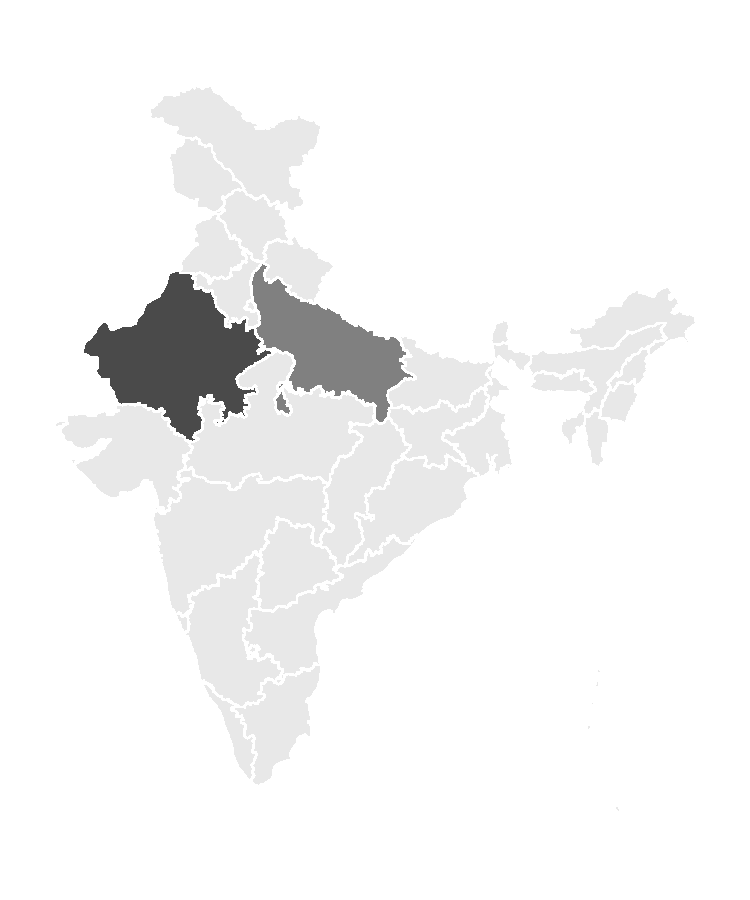
\includegraphics[width=\textwidth]{../figs/india_map_up_raj.pdf}
    
    \vspace{\medskipamount}
    
    \caption{Study States: Rajasthan and Uttar Pradesh}
    \label{fig:india_map}
    \vspace{\medskipamount}
    \parbox{0.9\textwidth}{\scriptsize
        \emph{Notes:} Highlighted states are the study sites. Rajasthan (darker grey, west): India's largest state by area (342,239 km\textsuperscript{2}), population 68.5 million (Census 2011), approximately 75\% rural, with 11,300 Gram Panchayats. Uttar Pradesh (lighter grey, east): India's most populous state, population 199.8 million (Census 2011), approximately 77\% rural, with 58,000 Gram Panchayats.
    }
\end{figure}
\section{Data and Research Design}
\subsection{Data}

We assemble four data sources for this study.

\paragraph{Electoral data.} We scraped GP-level election records from the Rajasthan and Uttar Pradesh State Election Commissions for four cycles each: 2005, 2010, 2015, and 2020 in Rajasthan, and 2005, 2010, 2015, and 2021 in UP. For each GP-election, we observe the reservation status of the Sarpanch seat (reserved for women, or open) and the sex of the elected Sarpanch. In Rajasthan 2015, the winner's sex was missing from official records and was manually coded from names. For Rajasthan 2020, we additionally collected candidate-level affidavit data (age, education, assets) from the SEC. Table~\ref{tab:gp_summary_combined} summarizes the electoral data. Between 2005 and 2020, the number of GPs in Rajasthan grew from roughly 9,200 to 11,500 ($\uparrow 25\%$), reflecting delimitation driven by population growth and urbanization. The number of Panchayat Samitis increased from 237 to 352 ($\uparrow 49\%$), while the number of districts was nearly constant, with only Pratapgarh added in 2008. In UP, the number of GPs, blocks, and districts remained approximately constant across cycles. As a validation check, we replicate the UP short-run results using independently collected data from \citet{weaver_data}.

\paragraph{Linking GPs across election cycles.} Constructing a panel of GPs across elections requires matching administrative units whose names vary over time due to transliteration inconsistencies, OCR errors in digitized records, and administrative renaming. We proceed in three steps. First, we standardize raw names within each election year using transliteration normalization (via the \texttt{stringi} package) and manual correction of OCR artifacts (e.g., ``JAW AJA'' $\rightarrow$ Jawaja, ``BANSW ARA'' $\rightarrow$ Banswara). Second, we construct validated crosswalks at each level of the administrative hierarchy. For districts, we manually map every raw election district name to its canonical SHRUG or LGD equivalent, handling spelling variants (Chittorgarh/Chittaurgarh), abbreviations (S. Madhopur/Sawai Madhopur), OCR errors, and post-2010 renamings (Allahabad $\rightarrow$ Prayagraj, Faizabad $\rightarrow$ Ayodhya). For sub-district units (Panchayat Samitis in Rajasthan, blocks in UP), we build analogous crosswalks to LGD block codes, achieving 100\% coverage of election units. In UP, this includes tracking blocks that moved between districts when Shamli, Sambhal, Hapur, and Amethi were carved out after 2010. Third, we match GPs across cycles by joining on normalized district-samiti-GP name strings, and manually verify a random sample of matches for accuracy.

\paragraph{Village-level covariates.} We link GPs to pre-treatment village characteristics via two additional data sources. The Local Government Directory (LGD), the Indian government's authoritative registry of rural administrative units, provides the mapping between GPs and census villages for 2020.\footnote{\url{https://lgdirectory.gov.in/}} We match election GPs to LGD GPs within each block using a combination of exact matching on normalized GP names and fuzzy string matching (Jaro-Winkler distance $< 0.20$) for remaining unmatched units. We use this mapping, together with the GP-to-LGD crosswalks described above, to join election data to village-level attributes from the Socioeconomic High-resolution Rural-Urban Geographic Platform for India (SHRUG 2.0; \citealp{asher2019socioeconomic}), which harmonizes data from the 1991 and 2001 Census Abstracts and Village Directories \citep{pcindia, chandramouli2011census}. We aggregate village-level covariates---population, female population, SC/ST composition, medical facilities, schools, water infrastructure, banking, power supply, and road access---to the GP level and use these for balance tests and covariate-adjusted specifications.

\paragraph{Phone audit data.} In 2024, we conducted a phone survey of Sarpanches elected in the 2020 Rajasthan elections, sampling separately from quota and open seats. We report these results separately in Section~\ref{sec:phone_audit}.

\subsection{Research Design}

Our estimand is the effect of reserving the Sarpanch position for women in one election on the probability that a woman wins in the subsequent election, conditional on the seat being open. We begin with the short-run analysis, where identification is most straightforward, then extend to cumulative exposure.

\subsubsection*{Short-run specification}

For each consecutive pair of elections, we estimate:

\begin{equation}\label{eq:estimation_eqn}
\text{FemaleWinner}_{g,t+1} = \beta \cdot \text{Quota}_{g,t} + \lambda_{d} + \varepsilon_{g,t+1},
\end{equation}

\noindent where $g$ indexes GPs, $\text{FemaleWinner}_{g,t+1}$ is an indicator for a woman winning the open seat in the next election, $\text{Quota}_{g,t}$ indicates whether GP $g$ was reserved for women in the current election, and $\lambda_d$ denotes district-samiti (Rajasthan) or district-block (UP) fixed effects. The sample is restricted to GPs whose seat is open in $t+1$. Standard errors are clustered by district--samiti in Rajasthan and district--block in UP, including models without fixed effects. We report all specifications with and without fixed effects and with and without pre-treatment village characteristics from the 2001 Census Village Directory, accessed via SHRUG 2.0 \citep{asher2019socioeconomic}. The coefficient $\beta$ is the intent-to-treat effect: the impact of having been reserved on the probability that a woman wins in the next open election. Our primary outcome is whether a woman wins. We also examine whether a woman contests, which speaks directly to the supply-side channel: if quotas expand the pipeline of female candidates, this should be visible in candidacy rates even if it does not translate into wins.

Note that this estimand captures the full causal chain from reservation to subsequent electoral outcomes, including any behavioral responses to the anticipated political environment. One might worry that candidates anticipate whether their seat will be open in the next cycle and adjust their behavior accordingly. A female Sarpanch who expects her seat to become unreserved may invest differently in building a political base than one who expects continued reservation. This concern exists under any assignment mechanism but is strongest when future open status is more predictable. It is not a threat to identification so long as anticipation is symmetric: the assignment rules are public information, and candidates in both reserved and open GPs can update their expectations about future reservation status.

Identification requires that quota assignment be independent of potential outcomes. Prior work treats assignment in these states as random or as-if random. In Rajasthan, assignment is reported to follow a lottery within each Panchayat Samiti \citep{chattopadhyay2004women, dunning2013ethnic, brule2023actually}. In Uttar Pradesh, assignment is described as following an administrative rule based on population size within blocks. We assess these claims directly.

Table~\ref{tab:balance_raj_2005_2010} reports descriptive balance and block-adjusted joint tests for Rajasthan. The clustered joint tests yield $p=0.17$, $0.09$, and $0.45$ across the three transitions. These tests do not establish the assignment mechanism or replace an assessment of the rotation rules.

In UP, the balance diagnostics show differences between quota and open GPs (Table~\ref{tab:balance_up_2005_2010}). We assess sensitivity using district--block fixed effects and five pre-treatment covariates: log population, SC share, literacy rate, female population share, and facility availability. Fixed effects absorb differences shared within a block; covariate adjustment does not establish that selection within blocks is ignorable.

Placebo tests regress the outcome in the prior election on quota status in the current election. Table~\ref{tab:placebo_combined} reports the resulting estimates and district--block clustered standard errors. The coefficients are not uniformly zero or statistically insignificant.

\subsubsection*{Rotation and its implications}

A complication arises from quota rotation. Both states shift quota assignments across election cycles: a GP reserved in one election is less likely to be reserved in the next (Tables~\ref{tab:treat_corr} and \ref{tab:long_term_treat_rotation}). In Rajasthan, the earliest transition (2005--2010) shows no rotation ($\hat{\beta} \approx 0.01$, $p > 0.3$), consistent with independent lottery draws. The chi-square test confirms independence ($\chi^2 = 1.80$, $p = 0.18$; Table~\ref{tab:chi_sq_raj}). Subsequent transitions show strong rotation ($\hat{\beta} = -0.40$ to $-0.29$, $p < 0.01$), indicating a policy shift after 2010. In UP, even the first transition shows modest rotation ($\hat{\beta} = -0.02$, $p < 0.01$), with stronger rotation in later periods. The chi-square test rejects independence for all transitions except 2005--2021 (Table~\ref{tab:chi_sq_up}). A four-way balanced panel restricted to GPs observed in all cycles yields nearly identical rotation coefficients (Appendix Table~\ref{tab:long_term_treat_rotation}).

Rotation matters for identification because we observe outcomes only for GPs whose seats are open in the next election. Since rotation links past quota status to future open status, conditioning on the seat being open is conditioning on a post-treatment variable. This is harmless if rotation is purely mechanical, determined by prior quota status alone and orthogonal to GP characteristics that predict female electoral success. It becomes a threat if rotation is confounded. If, for instance, larger or more developed GPs are systematically rotated out of reservation earlier, conditioning on open status could induce collider bias.

The balance evidence bears on this question. In Rajasthan, covariate balance remains strong even in the later panels where rotation is heaviest, suggesting that rotation does not operate through observable GP characteristics. In UP, the small standardized differences and stable estimates across specifications with and without controls point to the same conclusion. To assess this more directly, we conduct chi-square tests of independence between current and prior quota assignment at the district level, identifying districts where rotation appears consistent with independent draws and districts where it does not. We then restrict the sample to districts where the chi-square test does not reject independence and re-estimate Equation~\ref{eq:estimation_eqn}. Results are similar on these subsets (Tables~\ref{tab:chi_sq_raj} and \ref{tab:chi_sq_up}), providing further evidence that rotation-induced selection is not driving our findings.

\subsubsection*{Cumulative exposure}

The short-run specification asks whether a single cycle of reservation increases women's chances of winning in the next open election. A natural extension is whether repeated exposure compounds: does a GP reserved in two or three prior cycles show larger effects than one reserved in only one? We estimate effects of quota assignment in 2005 on outcomes in 2015 or 2020/2021, restricting to GPs open in the outcome year. We also estimate a treatment intensity specification that includes quota assignment indicators for multiple prior cycles and their interactions, recovering the marginal effect of each additional cycle of reservation. Identification here rests on the same assignment mechanism as the short-run analysis, but is complicated by the fact that cumulative exposure is partly a function of rotation patterns across intervening cycles. Because rotation is non-random in many districts after 2010, we also restrict the cumulative analysis to districts where chi-square tests do not reject independence of quota assignment across cycles. We report the historical 2015 restriction separately and compare the main cumulative specification at the same 2020/2021 horizon. Passing an independence test does not establish exogeneity. We treat the cumulative results throughout as informative about dose-response but less definitive than the short-run estimates.

\subsubsection*{Power and replication}

Approximate minimum detectable effects at 80\% power are \shortMdeMin{}--\shortMdeMax{} percentage points for the main short-run models (Appendix Table~\ref{tab:power_analysis}). Cumulative contrasts are less precise. We also replicate the UP short-run analysis using independently collected data from \citet{weaver_data}.

\section{Results}\label{sec:results}

\subsection{Short-run Effects}

Table~\ref{tab:short_term_main} reports estimates of Equation~\ref{eq:estimation_eqn} for each short-run panel, with and without district-samiti (Rajasthan) or district-block (UP) fixed effects. The outcome is whether a woman wins an open GP seat in the next election; the treatment is quota assignment in the current election.\footnote{Gender quotas are implemented alongside caste quotas. In seats with both caste and gender quotas, only women from the reserved caste group may contest. In seats with only a caste quota (no gender quota), both men and women from the reserved caste group may contest. Our results indicate that when a seat loses its gender quota, women are not substantially winning or contesting regardless of caste category.}

In Rajasthan, the fixed-effects estimates are \rajShortOne{}, \rajShortTwo{}, and \rajShortThree{} percentage points for the three successive transitions. Their district--samiti clustered 95\% confidence intervals are [\rajShortOneLow{}, \rajShortOneHigh{}], [\rajShortTwoLow{}, \rajShortTwoHigh{}], and [\rajShortThreeLow{}, \rajShortThreeHigh{}] points. In UP, the corresponding estimates are \upShortOne{}, \upShortTwo{}, and \upShortThree{} points, with district--block clustered intervals [\upShortOneLow{}, \upShortOneHigh{}], [\upShortTwoLow{}, \upShortTwoHigh{}], and [\upShortThreeLow{}, \upShortThreeHigh{}]. Appendix Table~\ref{tab:short_term_bootstrap} reports wild cluster bootstrap inference.

The negative Rajasthan estimate for 2010$\rightarrow$2015 warrants comment. This is the first transition where strong rotation appears ($\hat{\beta} = -0.41$ for lagged quota predicting current quota; Table~\ref{tab:treat_corr}). When we restrict to the eight districts (of 33) where within-district chi-squared tests fail to reject independence of quota assignment, the estimate flips to $+2$ percentage points (Table~\ref{tab:short_term_random_rotation}), though the restricted sample ($N = 777$) lacks power. The negative full-sample estimate thus likely reflects compositional differences between quota and open GPs introduced by non-random rotation, not a genuine backlash effect of quotas.

The UP effects are small in absolute terms, relative to control means of about 14--19\% and the 17.9 percentage point estimate in urban Mumbai reported by \citet{bhavnani2009electoral}. The short-run confidence intervals exclude an effect of that size. Approximate minimum detectable effects are \shortMdeMin{}--\shortMdeMax{} points at 80\% power (Appendix Table~\ref{tab:power_analysis}); this precision does not extend to every cumulative contrast or restricted sample.

\begin{table}[!htbp]
    \centering
    \caption{Short-run Effects}
    \label{tab:short_term_main}
    
\begingroup
\centering
\scriptsize
\begin{adjustbox}{max width=\linewidth}
   \begin{threeparttable}[b]
      \begin{tabular}{lcccccccccccc}
         \toprule
          & \multicolumn{6}{c}{Rajasthan} & \multicolumn{6}{c}{Uttar Pradesh} \\ 
          & \multicolumn{2}{c}{05$\rightarrow$10} & \multicolumn{2}{c}{10$\rightarrow$15} & \multicolumn{2}{c}{15$\rightarrow$20} & \multicolumn{2}{c}{05$\rightarrow$10} & \multicolumn{2}{c}{10$\rightarrow$15} & \multicolumn{2}{c}{15$\rightarrow$21} \\ 
                               & No FE        & FE            & No FE        & FE            & No FE        & FE            & No FE        & FE            & No FE        & FE            & No FE        & FE \\   
                               & [i]          & [ii]          & [iii]        & [iv]          & [v]          & [vi]          & [vii]        & [viii]        & [ix]         & [x]           & [xi]         & [xii]\\  
         \midrule 
         Intercept             & 0.09$^{***}$ &               & 0.09$^{***}$ &               & 0.12$^{***}$ &               & 0.13$^{***}$ &               & 0.15$^{***}$ &               & 0.19$^{***}$ &   \\   
                               & (0.007)      &               & (0.01)       &               & (0.010)      &               & (0.004)      &               & (0.004)      &               & (0.004)      &   \\   
         $\text{Quota}_{t-1}$  & 0.01         & 0.01          & -0.02$^{*}$  & -0.03$^{**}$  & 0.005        & 0.004         & 0.02$^{***}$ & 0.02$^{***}$  & 0.02$^{***}$ & 0.02$^{***}$  & 0.04$^{***}$ & 0.04$^{***}$\\   
                               & (0.009)      & (0.009)       & (0.01)       & (0.01)        & (0.01)       & (0.01)        & (0.005)      & (0.004)       & (0.005)      & (0.005)       & (0.005)      & (0.005)\\   
          \\
         R$^2$                 & 0.0006       & 0.10          & 0.001        & 0.15          & 0.00006      & 0.12          & 0.0008       & 0.06          & 0.0005       & 0.05          & 0.002        & 0.05\\  
         Observations          & 4,061        & 4,061         & 3,867        & 3,867         & 4,014        & 4,014         & 28,002       & 28,002        & 25,963       & 25,963        & 30,975       & 30,975\\  
          \\
         (District, Samiti) FE &              & $\checkmark$  &              &               &              &               &              &               &              &               &              & \\  
         (District, Samiti) FE &              &               &              & $\checkmark$  &              &               &              &               &              &               &              & \\  
         (District, Samiti) FE &              &               &              &               &              & $\checkmark$  &              &               &              &               &              & \\  
         (District, Block) FE  &              &               &              &               &              &               &              & $\checkmark$  &              &               &              & \\  
         (District, Block) FE  &              &               &              &               &              &               &              &               &              & $\checkmark$  &              & \\  
         (District, Block) FE  &              &               &              &               &              &               &              &               &              &               &              & $\checkmark$\\   
         \bottomrule
      \end{tabular}
      
      \begin{tablenotes}
         \item $^{***}$p$<$0.01; $^{**}$p$<$0.05; $^{*}$p$<$0.1. Outcome: woman elected in open seat. Sample restricted to GPs where seat was not reserved for women in outcome year. Standard errors clustered by district-samiti (Rajasthan) or district-block (UP).
      \end{tablenotes}
   \end{threeparttable}
\end{adjustbox}
\par\endgroup



\end{table}

\subsection{Cumulative Exposure}
 
If quotas generate lasting change through gradual erosion of discrimination and incremental pipeline expansion, the effects should grow with repeated exposure. We test this using the full interaction model, regressing whether a woman wins an open seat in the final election (2020 in Rajasthan, 2021 in UP) on quota status in each prior election and all two- and three-way interactions. Table~\ref{tab:long_run_interaction} reports the results.

In Rajasthan, reserving a GP in all three prior elections rather than none is associated with a \rajFullAlways{} percentage point increase in the probability of a woman winning the open seat in 2020. This compares \rajFullAlwaysLeftN{} GPs reserved in all three elections with \rajFullAlwaysRightN{} never reserved; the full model contains \rajFullAlwaysN{} GPs, and \rajFullAlwaysSharedClusters{} samitis contain both histories. The wild cluster bootstrap 95\% interval is [\rajFullAlwaysLow{}, \rajFullAlwaysHigh{}] points. Relative to reservation only in 2015, the contrast is \rajFullExtra{} points [\rajFullExtraLow{}, \rajFullExtraHigh{}]. These are linear combinations of the fitted coefficients, with uncertainty calculated using their full covariance matrix (Appendix Table~\ref{tab:cumulative_contrasts}).

In UP, three prior reservations versus none give \upFullAlways{} percentage points [\upFullAlwaysLow{}, \upFullAlwaysHigh{}], based on \upFullAlwaysLeftN{} versus \upFullAlwaysRightN{} GPs (\upFullAlwaysN{} in the full model; \upFullAlwaysSharedClusters{} blocks contain both histories). Three versus reservation only in 2015 give \upFullExtra{} points [\upFullExtraLow{}, \upFullExtraHigh{}]. The contrasts between two prior reservations that include 2015 and reservation only in 2015 remain small and imprecise. Table~\ref{tab:cumulative_contrasts} reports these comparisons directly; the signs of individual interaction terms cannot establish them on their own.
 
The three-way interaction remains positive. The resulting pattern need not represent a gradual dose-response relationship: GPs reserved in all three prior elections may differ from GPs with other histories because later open-seat status and the treatment history depend on the rotation process.
 
To compare the same outcome horizon, we retain the 2020 Rajasthan and 2021 UP outcomes when restricting to districts that pass independence tests for both the 2005--2010 and 2010--2015 transitions. The three-versus-zero contrasts are \rajRestrictedAlways{} points [\rajRestrictedAlwaysLow{}, \rajRestrictedAlwaysHigh{}] in Rajasthan ($N=\rajRestrictedAlwaysN{}$) and \upRestrictedAlways{} points [\upRestrictedAlwaysLow{}, \upRestrictedAlwaysHigh{}] in UP ($N=\upRestrictedAlwaysN{}$). In UP, the three-versus-one contrast is \upRestrictedExtra{} points [\upRestrictedExtraLow{}, \upRestrictedExtraHigh{}]. The wider intervals show the loss of precision; the point estimates do not collapse to zero. No UP districts pass tests for all three transitions, so that stricter restriction is unavailable.
 
The cumulative comparisons are positive in the full sample, and the restricted comparisons are less precise. Failing to reject independence within a district does not establish random assignment; these restrictions probe sensitivity to the observed rotation pattern.
 
\begin{table}[!htbp]
    \centering
    \caption{Cumulative Exposure Effects}
    \label{tab:long_run_interaction}
    
\begingroup
\centering
\scriptsize
\begin{adjustbox}{max width=\linewidth}
   \begin{threeparttable}[b]
      \begin{tabular}{lcccc}
         \toprule
          & \multicolumn{2}{c}{Rajasthan} & \multicolumn{2}{c}{Uttar Pradesh} \\ 
                                                                                                  & No FE        & FE            & No FE        & FE \\   
                                                                                                  & [i]          & [ii]          & [iii]        & [iv]\\  
         \midrule 
         Intercept                                                                                & 0.08$^{***}$ &               & 0.17$^{***}$ &   \\   
                                                                                                  & (0.02)       &               & (0.008)      &   \\   
         $\text{Quota}_{2005}$                                                                    & -0.02        & 0.00003       & 0.02$^{*}$   & 0.02$^{*}$\\   
                                                                                                  & (0.03)       & (0.03)        & (0.01)       & (0.01)\\   
         $\text{Quota}_{2010}$                                                                    & 0.05$^{**}$  & 0.07$^{***}$  & 0.008        & 0.007\\   
                                                                                                  & (0.02)       & (0.02)        & (0.01)       & (0.01)\\   
         $\text{Quota}_{2015}$                                                                    & 0.02         & 0.04$^{*}$    & 0.04$^{***}$ & 0.05$^{***}$\\   
                                                                                                  & (0.02)       & (0.02)        & (0.01)       & (0.01)\\   
         $\text{Quota}_{2005}$ $\times$ $\text{Quota}_{2010}$                                     & 0.04         & 0.02          & -0.02        & -0.02\\   
                                                                                                  & (0.04)       & (0.04)        & (0.02)       & (0.02)\\   
         $\text{Quota}_{2005}$ $\times$ $\text{Quota}_{2015}$                                     & 0.06         & 0.03          & -0.01        & -0.02\\   
                                                                                                  & (0.04)       & (0.04)        & (0.02)       & (0.02)\\   
         $\text{Quota}_{2010}$ $\times$ $\text{Quota}_{2015}$                                     & -0.02        & -0.05         & 0.004        & -0.003\\   
                                                                                                  & (0.03)       & (0.03)        & (0.02)       & (0.02)\\   
         $\text{Quota}_{2005}$ $\times$ $\text{Quota}_{2010}$ $\times$ $\text{Quota}_{2015}$      & -0.04        & -0.02         & 0.08$^{**}$  & 0.09$^{***}$\\   
                                                                                                  & (0.05)       & (0.05)        & (0.03)       & (0.03)\\   
          \\
         R$^2$                                                                                    & 0.006        & 0.14          & 0.005        & 0.06\\  
         Observations                                                                             & 2,671        & 2,671         & 14,117       & 14,117\\  
          \\
         (District, Samiti) FE                                                                    &              & $\checkmark$  &              & \\  
         (District, Block) FE                                                                     &              &               &              & $\checkmark$\\   
         \bottomrule
      \end{tabular}
      
      \begin{tablenotes}
         \item $^{***}$p$<$0.01; $^{**}$p$<$0.05; $^{*}$p$<$0.1. The dependent variable is whether a woman was elected in an open seat (2020 for Rajasthan, 2021 for UP). Sample restricted to GPs where seat was not reserved for women in outcome year. Treatment variables indicate quota status in each prior election year. Standard errors clustered by district-samiti (Rajasthan) or district-block (UP).
      \end{tablenotes}
   \end{threeparttable}
\end{adjustbox}
\par\endgroup



\end{table}


\subsection{Candidacy Effects}

Quotas might affect electoral dynamics through candidacy rather than winning \citep{o2020can, auerbach2016electoral}. Even if more women do not win once quotas are withdrawn, quotas might encourage more women to contest when the seat becomes open. We test this using candidate-level data from the 2020 Rajasthan elections, estimating the full interaction model on four outcomes: the proportion of candidates who are women, the number of women candidates, whether at least one woman ran, and women's vote share among the top two candidates.

Table~\ref{tab:candidacy_combined} reports the results. Candidate counts and sex are linked within the same 2020 general-election phase and GP. The vote outcome is the number of votes cast for women among the winner and runner-up divided by all valid votes, not the share among only those two candidates. None of the quota or treatment-history coefficients is statistically significant at the 5\% level in these specifications. The three-way interactions remain imprecise.

\section{Robustness}\label{sec:robustness}

\paragraph{Covariate adjustment.} We add log population, SC share, literacy rate, female population share, and facility availability to the short-run models on the matched Census sample (Table~\ref{tab:shrug_covariates}). With fixed effects, the Rajasthan 2005--2010 estimate is 1.7 percentage points ($p=.20$), the Rajasthan 2010--2015 estimate is $-3.1$ points ($p=.02$), and the UP 2005--2010 estimate is 0.9 points ($p=.20$). Adjustment also restricts the sample to GPs with the required observed covariates.

\paragraph{Random-rotation district restriction.} Table~\ref{tab:short_term_random_rotation} restricts to districts where descriptive tests do not reject independence of consecutive quota assignments. Rajasthan retains 32, 8, and 12 districts across the three transitions, while UP retains 48, 14, and none. The Rajasthan 2015--2020 fixed-effects estimate is 0.8 percentage points; the restriction does not support a claim that it is exactly zero. No UP 2015--2021 model can be estimated under this restriction. The cumulative comparison uses the same final election as the main specification (Table~\ref{tab:cumulative_contrasts}); the historical 2015 outcome is reported separately.

\paragraph{Placebo tests.} Table~\ref{tab:placebo_combined} tests whether future quota status predicts past outcomes. The estimates are not all zero, and some depend on the inclusion of fixed effects. These diagnostics do not establish exogeneity of the reservation process.

\paragraph{Replication with independent data.} We replicate the UP analyses using independently collected data from \citet{weaver_data}, collected for \citet{narasimhan2024polity}, which covers 2010, 2015, and 2021 elections (the last wave is coded 2020 in the source) with substantially larger samples ($N \approx 37{,}000$--$39{,}000$). The short-run estimates (Table~\ref{tab:weaver_short}) are 2 percentage points for 2010$\rightarrow$2015 ($p < 0.01$) and 4 percentage points for 2015$\rightarrow$2021 ($p < 0.01$), matching our main UP results. These models use 2011 Census district--block identifiers for fixed effects and clustering because the source election-specific block fields are unavailable for the matched 2010--2015 sample. The cumulative exposure interaction model (Table~\ref{tab:weaver_long}) shows a significant 2015 quota effect (4 percentage points, $p < 0.01$) with an interaction of approximately 0.6 percentage points that is not statistically significant, consistent with our finding that the most recent quota drives the result in UP.

\section{Why Women Do Not Win or Run}\label{sec:mechanisms}

The short-run and cumulative estimates differ in magnitude and precision. We now examine the institutional environment that may help explain these patterns.

\subsection{Male Proxy Governance}\label{sec:phone_audit}

The channels through which quotas are theorized to generate lasting representation all require that women elected under quotas actually exercise political authority. To measure who exercises day-to-day authority, we conducted a phone audit exploiting a feature of Indian local politics: elected representatives extensively use mobile phones for citizen engagement, a practice documented in media accounts \citep{rigillo2018whatsapp} and confirmed in our interviews with political staff.\footnote{Author's phone interview with former secretarial staff (name and affiliation withheld on request), December 20, 2024.} We scraped official electoral records from the Rajasthan State Election Commission containing the self-reported mobile phone numbers of all 2020 winners.\footnote{The study protocol was reviewed by the IRB under protocol number UP-24-00498.} We block-sampled 500 Sarpanches from seats reserved for women across districts and contacted them between July and August 2024, with the average call lasting about one minute.

Panel A of Table~\ref{tab:full_survey} reports the results. Of 500 records, 377 (75\%) had an answered call; 35 (9.3\%) were recorded as answered by the elected representative. Male non-members answered 319 calls (84.6\%): 172 were spouses, 46 children, and 44 other recorded relatives. The remaining 57 had no recorded relationship (56) or were inconsistently coded as ``self'' (1). Six respondents were female non-members, six were non-members with unavailable sex, and eleven had unavailable identity. Among 331 non-member respondents, 283 did not transfer the call and three did; transfer status was unavailable for 43 and recorded as not applicable for two.

Two cases illustrate the pattern. In one, the elected representative initially answered but transferred the call to her spouse when we began asking about panchayat governance. In another, a father-in-law answered and insisted that he was the ``Pratinidhi'' (representative).

To benchmark these patterns, we contacted 507 randomly sampled representatives from open seats using the same protocol. The response rate was 79\% (400 of 507). In open seats, 76.2\% of answered calls reached the elected representative directly (Panel B of Table~\ref{tab:full_survey}). A citizen calling a quota-seat representative speaks with the actual officeholder less than one in ten times; a citizen calling an open-seat representative does so three quarters of the time.

Linking the open-seat call sheet to unique election-phase, district, samiti, and winner-name records identifies 63 female-held seats, of which 46 had answered calls. Fourteen calls were recorded as answered by the representative, but seven of those respondents were coded male. The call notes also identify these respondents as the member and do not resolve the conflict. Thus 7--14 of the 46 calls (15--30\%) are consistent with direct contact if the only disputed records are these seven. Sixteen of the 507 sampled records have unresolved officeholder sex. These records do not support a precise estimate of direct contact with women in open seats.

\begin{table}[!htbp]
    \centering
    \caption{Phone Audit Response Distribution}
    \label{tab:full_survey}
    \setlength{\tabcolsep}{4pt}

    \begin{subtable}[t]{0.45\linewidth}
        \centering\scriptsize
        \caption*{\textbf{Panel A: Gender-Quota Seats}}
        
\begin{tabular}[t]{lr}
\toprule
Category & N (\%)\\
\midrule
\addlinespace[0.3em]
\multicolumn{2}{l}{\textit{Initial contact}}\\
Answered & 377 (75.4)\\
No answer recorded & 123 (24.6)\\
\addlinespace[0.3em]
\multicolumn{2}{l}{\textit{Among answered}}\\
Recorded as elected representative & 35 (9.3)\\
Male non-member & 319 (84.6)\\
Female non-member & 6 (1.6)\\
Non-member, sex unavailable & 6 (1.6)\\
Identity unavailable & 11 (2.9)\\
\addlinespace[0.3em]
\multicolumn{2}{l}{\textit{Among male non-members}}\\
Child & 46 (14.4)\\
Other recorded relative & 44 (13.8)\\
Relationship recorded as self & 1 (0.3)\\
Relationship unavailable & 56 (17.6)\\
Spouse & 172 (53.9)\\
\addlinespace[0.3em]
\multicolumn{2}{l}{\textit{Among non-members}}\\
Did not transfer & 283 (85.5)\\
Transfer recorded as not applicable & 2 (0.6)\\
Transfer status unavailable & 43 (13.0)\\
Transferred & 3 (0.9)\\
\bottomrule
\end{tabular}

    \end{subtable}
    \hspace{2em}
    \begin{subtable}[t]{0.45\linewidth}
        \centering\scriptsize
        \caption*{\textbf{Panel B: Open Seats}}
        
\begin{tabular}[t]{lr}
\toprule
Category & N (\%)\\
\midrule
\addlinespace[0.3em]
\multicolumn{2}{l}{\textit{Initial contact}}\\
Answered & 400 (78.9)\\
No answer recorded & 107 (21.1)\\
\addlinespace[0.3em]
\multicolumn{2}{l}{\textit{Among answered}}\\
Recorded as elected representative & 305 (76.2)\\
Male non-member & 66 (16.5)\\
Female non-member & 10 (2.5)\\
Non-member, sex unavailable & 3 (0.8)\\
Identity unavailable & 16 (4.0)\\
\bottomrule
\end{tabular}

    \end{subtable}

    \vspace{\medskipamount}

    \parbox{0.9\textwidth}{\scriptsize
        \emph{Notes:} Phone audit of elected Sarpanches in Rajasthan. We attempted to contact each representative up to three times between 10:00 am and 6:30 pm, conducting the conversation in Hindi. In addition to noting the initial point of contact, we asked respondents about their previous electoral experience, family involvement in politics, regularity of gram sabha meetings, and attendance at these meetings. The survey script is provided in Appendix Section~\ref{sec:phone_survey_script}.

        \medskip

        \emph{Panel A:} 500 quota-seat call records across Rajasthan, contacted July--August 2024 (average call duration: one minute).

        \medskip

        \emph{Panel B:} 507 open-seat call records across Rajasthan, contacted August--December 2024.
    }
\end{table}

If male relatives perform the representative function in the vast majority of quota seats, voters cannot observe female leadership, women in office cannot accumulate governing experience, and other potential female candidates observe family power rather than female political competence. The 2008 Panchayati Raj Ministry report finds that over 89\% of women representatives did not contest another election after their term \citep[pp.~26, 63]{ministry2008}, consistent with officeholders who never governed in practice having no basis on which to build a political career. These findings complement work by \citet{cheema2020canvassing, khan2021count, prillaman2023strength} and \citet{kumar2024} on male household members as constraints on women's political participation.

A concern is that gender gaps in mobile phone ownership, rather than proxy governance, drive the results. Rural phone ownership rates differ substantially by sex: 81\% for men aged 15--49 versus 57\% for women \citep[Fig.~2.2, p.~7]{mospi2025mobile}. Two features of our setting mitigate this concern. First, the phone numbers we call are self-reported by candidates in officially sworn affidavits filed under Section 125A of India's Representation of the People Act, 1951, which prohibits false or concealed information under penalty of imprisonment \citep[p.~52]{india_rpa_1951}. Phone ownership among political elites filing such affidavits likely exceeds population rates. Second, the contrast between quota seats (9\% representative answers) and open seats (76\% representative answers) is too large to be explained by differential phone ownership alone. What we cannot rule out is that women politicians are systematically less likely than men to answer calls from unknown numbers. Evidence on this specific behavior among political elites does not exist to our knowledge. Phone interception also captures only one dimension of proxy governance; male control likely extends to other spheres of political work, including gram sabha meetings, interactions with block officials, and disbursement decisions, that our audit cannot observe.

\subsection{Candidate Characteristics}\label{sec:cand_char}

Proxy governance is not the only barrier. The composition of the candidate pool under quotas may itself weaken the exposure mechanism. If quota-elected women are less professionalized than open-seat winners on dimensions that voters associate with competence, even voters who do interact with the officeholder may not update positively \citep{hansen1997talking, atkeson2003not, weeks2015quotas}.

Table~\ref{tab:main_cand_char} compares observable characteristics of winners and candidates in quota versus open seats in the 2020 Rajasthan elections, using data from officially sworn candidate affidavits. Winners in open seats are about 1.6 years older than winners in quota seats ($p < 0.01$), have 11 percentage points higher graduation rates (24\% vs.\ 12\%, $p < 0.01$), own more assets (log assets \allLogassetsOpen{} vs.\ \allLogassetsQuota{}, $p < 0.01$), and are far less likely to report being unemployed (10\% vs.\ 61\%, $p < 0.01$). These patterns hold across the full candidate pool: all-candidate comparisons show nearly identical gaps. Similar patterns appear in UP (Table~\ref{tab:up_cand_char}): open-seat winners are older, more educated, and (where available) wealthier than quota-seat winners, with the education gap narrowing slightly over time.

\begin{table}
\centering
\caption{\label{tab:main_cand_char}Candidate Characteristics: Quota vs. Open Seats (Rajasthan 2020)}
\centering
\fontsize{8}{10}\selectfont
\begin{threeparttable}
\begin{tabular}[t]{lrrrrrr}
\toprule
\multicolumn{1}{c}{ } & \multicolumn{3}{c}{Winners} & \multicolumn{3}{c}{Candidates} \\
\cmidrule(l{3pt}r{3pt}){2-4} \cmidrule(l{3pt}r{3pt}){5-7}
Characteristic & Open & Quota & Difference & Open & Quota & Difference\\
\midrule
Age & 42.79 & 41.18 & 1.61 & 41.50 & 39.83 & 1.67\\
Children & 2.06 & 2.14 & -0.08 & 1.90 & 2.03 & -0.12\\
Graduate & 0.24 & 0.12 & 0.11 & 0.22 & 0.13 & 0.09\\
Unemployed & 0.10 & 0.61 & -0.51 & 0.11 & 0.61 & -0.51\\
Log assets & 12.93 & 12.56 & 0.37 & 12.33 & 12.07 & 0.26\\
\bottomrule
\end{tabular}
\begin{tablenotes}
\item \textit{Note: } 
\item Descriptive open-minus-quota comparisons, conditional on candidacy or winning. Assets winsorized at the 10th and 90th percentiles of the candidate sample before taking logs. These comparisons do not identify a causal effect on candidate quality.
\end{tablenotes}
\end{threeparttable}
\end{table}


The all-winner comparison also reflects the different sex composition of quota and open seats. Among women winners, graduation rates are \womenGraduateOpen{}\% in open seats and \womenGraduateQuota{}\% in quota seats; mean log assets are \womenLogassetsOpen{} and \womenLogassetsQuota{}. Unemployment rates are \womenUnemployedOpen{}\% and \womenUnemployedQuota{}\%. Appendix Table~\ref{tab:candidate_women} reports women-only comparisons. Both sets are descriptive comparisons conditional on candidacy or winning.

The unemployment gap deserves a caveat: self-reported unemployment is shaped by gender norms, with men potentially less likely to classify themselves as unemployed even when not formally employed. Still, the composite picture across age, education, and assets points in the same direction: women elected under quotas are less professionalized on observable dimensions.

Among the 35 quota-elected representatives who answered our phone calls (out of 377), respondents are younger (mean age 37.4) and more likely to be employed than the broader quota-winner population (Table~\ref{tab:phone_reply_char}). This is consistent with women who actually exercise political authority being a positively selected subset of those who hold office under quotas.

These patterns align with the 2008 Panchayati Raj Ministry report \citep[pp.~26, 63]{ministry2008} and earlier studies \citep[Table~VII]{chattopadhyay2004women, ban2008tokenism, raabe2009effects}. \citet[Tables~5--6]{gajwani2015gender} find comparable education levels but document knowledge disparities and less contact with higher-level officials among quota-elected women. The candidate characteristics we observe may also reflect the broader pool of women willing to contest under quotas, potentially leading to lower average qualifications as the pool expands \citep{bhavnani2024does}.

The two findings reinforce each other. Less professionalized candidates are more susceptible to proxy governance: a woman with less education, fewer assets, and less labor market experience is less likely to resist her husband or father-in-law taking over the representative function. And proxy governance prevents the officeholder from acquiring the experience that would professionalize her, trapping quota-seat women in a cycle where the preconditions for lasting change are never established.

\subsection{Does Development Moderate the Quota Effect?}\label{sec:het_effects}

A natural explanation for the contrast between our findings and the large effects reported by \citet{bhavnani2009electoral} in urban Mumbai is that development moderates the quota effect. In more urbanized, better-connected settings, the barriers we document may be weaker: voters are more likely to have encountered women in professional roles, the female candidate pool may be deeper and more professionalized, and household structures may be less patriarchal. If this account is correct, quota effects should increase along the development gradient within our sample.

We test this by interacting the quota treatment with three GP-level markers of development drawn from the 2001 Census Village Directory (via SHRUG): the mean recorded village-to-town distance across constituent villages (above vs.\ below the GP median), an infrastructure index (whether the number of facility types available in at least one constituent village exceeds the median), and female literacy rate (above vs.\ below median). Cutoffs use matched GPs with observed covariates before restricting by the election outcome. Facility absence requires observed absence in every constituent village; unavailable means remain missing. We also use the minimum recorded village-to-town distance as a sensitivity analysis.

Table~\ref{tab:het_effects} reports the results for all six short-run panels. None of the 18 treatment-by-development interaction terms is significant at the 5\% level with district--block clustering. The same holds when proximity uses the minimum recorded village-to-town distance. Estimates and samples change when facility availability and missing covariates are handled consistently.

These within-rural comparisons do not provide clear evidence of moderation by the measured covariates. Their uncertainty does not rule out meaningful differences, and the comparisons do not identify the reason for the gap with Mumbai.

\section{Conclusion}\label{sec:conclusion}

Across four election cycles in each state, short-run estimates are small relative to the Mumbai benchmark. Three prior reservations versus none yield larger positive contrasts: \rajFullAlways{} percentage points in Rajasthan and \upFullAlways{} in UP. Restrictions based on observed rotation patterns reduce precision without demonstrating that these cumulative associations disappear. Their causal interpretation depends on the assignment and selection issues discussed above.

Our phone audit and candidate data point to why. In rural Rajasthan, only 9\% of calls to quota-seat Sarpanches reached the elected representative; 85\% were answered by male non-members, including 69\% explicitly recorded as relatives. Without direct citizen interaction with female leaders, the channels through which quotas are theorized to build lasting representation have nothing to work with. Women elected under quotas are also less professionalized than open-seat winners: younger, less educated, less wealthy, and far more likely to report being unemployed. These gaps compound the proxy governance problem, as less professionalized candidates are more susceptible to male relatives taking over the representative function.

We cannot adjudicate between all competing explanations for these results. Quotas may delegitimize women politicians, whom voters perceive as beneficiaries of a mandate rather than competitive candidates \citep[p.~111]{krook2006gender}. Taste-based discrimination may prevent women from winning open seats regardless of their performance \citep{desai2024women}. Our data are consistent with these accounts but do not isolate them from the proxy governance and candidate professionalization channels.

A suggestive piece of evidence on scope conditions comes from extending the phone audit to urban Jaipur, where 31.7\% of calls to quota-seat representatives reached the elected officeholder, compared with 9.3\% in rural areas (Table~\ref{tab:jaipur_quota}). Proxy governance is less prevalent in urban settings, though it remains the norm even there. This gradient is consistent with the gap between our rural results and \citet{bhavnani2009electoral}'s large urban effects, and suggests that the conditions under which quotas generate lasting representation are more likely to be met where household structures, labor markets, and women's public-sphere participation differ from rural India.

The policy implication is not that quotas are ineffective. Quotas guarantee descriptive representation, and compliance with India's mandate has placed nearly a million women in elected local office. The implication is that quotas alone are insufficient to create the conditions for women to retain political power independently. The binding constraint is not the absence of a legal mandate but the persistence of household-level power structures that quotas do not reach. Complementary interventions that address proxy governance directly, whether through transparency requirements, training programs that build women's independent political networks, or enforcement mechanisms that ensure elected women exercise their authority, may be necessary for quotas to fulfill their transformative potential.

\clearpage
\newpage
\bibliographystyle{chicago-apsr}
\bibliography{quota_raj}

\clearpage
\newpage
\begin{center}
 \vspace{36pt}
\LARGE{Supplementary Information for ``The Limits of Electoral Gender Quotas in Rural Local
Bodies''}
\end{center}

\appendix
\doublespacing
\thispagestyle{empty}

% Reset numbering for tables and figures to use section-based prefixes (A1, B1, etc.)
\counterwithin{table}{section}
\counterwithin{figure}{section}
\renewcommand{\thetable}{\thesection\arabic{table}}
\renewcommand{\thefigure}{\thesection\arabic{figure}}

% Local TOC for appendix only
\renewcommand{\contentsname}{Appendix Contents}
\startcontents[appendix]
\printcontents[appendix]{}{1}{\setcounter{tocdepth}{2}}
\clearpage
\newpage

\doublespacing

% =============================================================================
% APPENDIX A: DATA AND RESEARCH DESIGN
% =============================================================================

\section{Data and Research Design}\label{sec:app_data}

\begin{table}[!h]
\centering
\caption{\label{tab:gp_summary_combined}Summary of Gram Panchayats by Election Year}
\centering
\fontsize{8}{10}\selectfont
\begin{threeparttable}
\begin{tabular}[t]{lrrrr}
\toprule
 & 2005 & 2010 & 2015 & 2020\\
\midrule
\addlinespace[0.3em]
\multicolumn{5}{l}{\textit{\textbf{Panel A: Rajasthan}}}\\
\hspace{1em}Gram Panchayats & 9,178 & 9,166 & 9,862 & 11,506\\
\hspace{1em}Panchayat Samitis & 237 & 249 & 300 & 352\\
\hspace{1em}Districts & 32 & 33 & 33 & 33\\
\hspace{1em}Women Reserved (\%) & 33.5 & 47.6 & 48.4 & 50.0\\
\addlinespace[0.3em]
\multicolumn{5}{l}{\textit{\textbf{Panel B: Uttar Pradesh}}}\\
\hspace{1em}Gram Panchayats & 51,737 & 41,227 & 58,994 & 49,772\\
\hspace{1em}Panchayat Samitis & 846 & 844 & 823 & 728\\
\hspace{1em}Districts & 70 & 72 & 75 & 67\\
\hspace{1em}Women Reserved (\%) & 50.0 & 50.0 & 50.0 & 50.0\\
\bottomrule
\end{tabular}
\begin{tablenotes}
\item \textit{Note: } 
\item GP counts represent the total number of Gram Panchayats for which we have electoral data. The number of GPs increased between 2010 and 2020 due to delimitation (redistricting). The 2020 column for UP contains 2021 election data.
\end{tablenotes}
\end{threeparttable}
\end{table}
\FloatBarrier
\begin{table}[!h]
\centering
\caption{\label{tab:state_local_totals}Women's Representation: State vs Local Government}
\centering
\fontsize{8}{10}\selectfont
\begin{threeparttable}
\begin{tabular}[t]{lrrr}
\toprule
Level of Government & Total Representatives & Women & \% Women\\
\midrule
\addlinespace[0.3em]
\multicolumn{4}{l}{\textit{\textbf{State Legislatures (1950--2024)}}}\\
\hspace{1em}All State Legislators & $\approx$ 40,000 & $\approx$ 2,000 & 5.0\\
\addlinespace[0.3em]
\multicolumn{4}{l}{\textit{\textbf{Local Bodies (Current)}}}\\
\hspace{1em}Gram Panchayats & $\approx$ 250,000 & --- & ---\\
\hspace{1em}Total Elected Representatives & $>$ 2,000,000 & $\approx$ 1,000,000 & $\approx$ 50.0\\
\bottomrule
\end{tabular}
\begin{tablenotes}
\item \textit{Note: } 
\item State legislature data compiled from historical records of all state elections since 1950. Local body data from the Ministry of Panchayati Raj and Local Government Directory (2024). The contrast illustrates how gender quotas have dramatically increased women's descriptive representation at the local level compared to higher levels where quotas are not mandated.
\end{tablenotes}
\end{threeparttable}
\end{table}
\FloatBarrier

% =============================================================================
% APPENDIX B: IDENTIFICATION
% =============================================================================

\clearpage
\section{Identification}\label{sec:app_identification}

Our identification strategy relies on the rotation mandate: once a GP is reserved for women, it cannot be reserved again in the subsequent election. We present four types of evidence on identification: treatment rotation regressions, chi-squared tests of independence, balance tests on prior electoral characteristics, and balance tests on pre-treatment census covariates.

\begin{table}[!htbp]
    \centering
    \caption{Treatment Rotation: Quota Assignment Correlation Across Election Cycles (2-Way Panel)}
    \label{tab:treat_corr}
    
\begingroup
\centering
\scriptsize
\begin{adjustbox}{max width=\linewidth}
   \begin{threeparttable}[b]
      \begin{tabular}{lcccccccccccc}
         \toprule
          & \multicolumn{6}{c}{Rajasthan} & \multicolumn{6}{c}{Uttar Pradesh} \\ 
          & \multicolumn{2}{c}{05$\rightarrow$10} & \multicolumn{2}{c}{10$\rightarrow$15} & \multicolumn{2}{c}{15$\rightarrow$20} & \multicolumn{2}{c}{05$\rightarrow$10} & \multicolumn{2}{c}{10$\rightarrow$15} & \multicolumn{2}{c}{15$\rightarrow$21} \\ 
                               & No FE        & FE            & No FE         & FE            & No FE         & FE            & No FE         & FE            & No FE         & FE            & No FE         & FE \\   
                               & [i]          & [ii]          & [iii]         & [iv]          & [v]           & [vi]          & [vii]         & [viii]        & [ix]          & [x]           & [xi]          & [xii]\\  
         \midrule 
         Intercept             & 0.47$^{***}$ &               & 0.67$^{***}$  &               & 0.62$^{***}$  &               & 0.34$^{***}$  &               & 0.38$^{***}$  &               & 0.43$^{***}$  &   \\   
                               & (0.005)      &               & (0.01)        &               & (0.01)        &               & (0.003)       &               & (0.002)       &               & (0.002)       &   \\   
         $\text{Quota}_{t-1}$  & 0.01         & 0.01          & -0.41$^{***}$ & -0.41$^{***}$ & -0.29$^{***}$ & -0.29$^{***}$ & -0.02$^{***}$ & -0.03$^{***}$ & -0.11$^{***}$ & -0.11$^{***}$ & -0.28$^{***}$ & -0.28$^{***}$\\   
                               & (0.01)       & (0.01)        & (0.03)        & (0.03)        & (0.03)        & (0.03)        & (0.006)       & (0.006)       & (0.006)       & (0.006)       & (0.004)       & (0.004)\\   
          \\
         R$^2$                 & 0.0001       & 0.01          & 0.16          & 0.17          & 0.08          & 0.10          & 0.0006        & 0.01          & 0.01          & 0.01          & 0.08          & 0.08\\  
         Observations          & 7,667        & 7,667         & 7,447         & 7,447         & 7,882         & 7,882         & 39,510        & 39,510        & 34,556        & 34,556        & 41,924        & 41,924\\  
          \\
         (District, Samiti) FE &              & $\checkmark$  &               &               &               &               &               &               &               &               &               & \\  
         (District, Samiti) FE &              &               &               & $\checkmark$  &               &               &               &               &               &               &               & \\  
         (District, Samiti) FE &              &               &               &               &               & $\checkmark$  &               &               &               &               &               & \\  
         (District, Block) FE  &              &               &               &               &               &               &               & $\checkmark$  &               &               &               & \\  
         (District, Block) FE  &              &               &               &               &               &               &               &               &               & $\checkmark$  &               & \\  
         (District, Block) FE  &              &               &               &               &               &               &               &               &               &               &               & $\checkmark$\\   
         \bottomrule
      \end{tabular}
      
      \begin{tablenotes}
         \item $^{***}$p$<$0.01; $^{**}$p$<$0.05; $^{*}$p$<$0.1. Outcome: quota status in election $t$. Treatment: quota status in election $t-1$. Sample includes all GPs (not restricted to open seats). A negative coefficient indicates rotation away from previously reserved GPs, consistent with the rotation mandate. Standard errors clustered by district-samiti (Rajasthan) or district-block (UP).
      \end{tablenotes}
   \end{threeparttable}
\end{adjustbox}
\par\endgroup



\end{table}

\begin{table}[!htbp]
    \centering
    \caption{Treatment Rotation: Quota Assignment Correlation Across Election Cycles (4-Way Panel)}
    \label{tab:long_term_treat_rotation}
    
\begingroup
\centering
\scriptsize
\begin{adjustbox}{max width=\linewidth}
   \begin{threeparttable}[b]
      \begin{tabular}{lcccccccccccc}
         \toprule
          & \multicolumn{6}{c}{Rajasthan} & \multicolumn{6}{c}{Uttar Pradesh} \\ 
          & \multicolumn{2}{c}{05$\rightarrow$10} & \multicolumn{2}{c}{10$\rightarrow$15} & \multicolumn{2}{c}{15$\rightarrow$20} & \multicolumn{2}{c}{05$\rightarrow$10} & \multicolumn{2}{c}{10$\rightarrow$15} & \multicolumn{2}{c}{15$\rightarrow$21} \\ 
                               & No FE        & FE            & No FE         & FE            & No FE         & FE            & No FE        & FE            & No FE         & FE            & No FE         & FE \\   
                               & [i]          & [ii]          & [iii]         & [iv]          & [v]           & [vi]          & [vii]        & [viii]        & [ix]          & [x]           & [xi]          & [xii]\\  
         \midrule 
         Intercept             & 0.46$^{***}$ &               & 0.68$^{***}$  &               & 0.64$^{***}$  &               & 0.34$^{***}$ &               & 0.38$^{***}$  &               & 0.44$^{***}$  &   \\   
                               & (0.007)      &               & (0.01)        &               & (0.01)        &               & (0.004)      &               & (0.003)       &               & (0.003)       &   \\   
         $\text{Quota}_{t-1}$  & 0.02         & 0.02          & -0.42$^{***}$ & -0.43$^{***}$ & -0.32$^{***}$ & -0.32$^{***}$ & -0.02$^{**}$ & -0.02$^{**}$  & -0.11$^{***}$ & -0.11$^{***}$ & -0.29$^{***}$ & -0.29$^{***}$\\   
                               & (0.01)       & (0.01)        & (0.03)        & (0.03)        & (0.03)        & (0.03)        & (0.008)      & (0.008)       & (0.008)       & (0.008)       & (0.006)       & (0.006)\\   
          \\
         R$^2$                 & 0.0003       & 0.03          & 0.18          & 0.19          & 0.10          & 0.12          & 0.0004       & 0.02          & 0.01          & 0.02          & 0.08          & 0.09\\  
         Observations          & 5,334        & 5,334         & 5,334         & 5,334         & 5,334         & 5,334         & 21,499       & 21,499        & 21,499        & 21,499        & 21,499        & 21,499\\  
          \\
         (District, Samiti) FE &              & $\checkmark$  &               &               &               &               &              &               &               &               &               & \\  
         (District, Samiti) FE &              &               &               & $\checkmark$  &               &               &              &               &               &               &               & \\  
         (District, Samiti) FE &              &               &               &               &               & $\checkmark$  &              &               &               &               &               & \\  
         (District, Block) FE  &              &               &               &               &               &               &              & $\checkmark$  &               &               &               & \\  
         (District, Block) FE  &              &               &               &               &               &               &              &               &               & $\checkmark$  &               & \\  
         (District, Block) FE  &              &               &               &               &               &               &              &               &               &               &               & $\checkmark$\\   
         \bottomrule
      \end{tabular}
      
      \begin{tablenotes}
         \item $^{***}$p$<$0.01; $^{**}$p$<$0.05; $^{*}$p$<$0.1. Outcome: quota status in election $t$. Treatment: quota status in election $t-1$. Sample includes GPs present in all four election years (4-way panel). A negative coefficient indicates rotation away from previously reserved GPs, consistent with the rotation mandate. Standard errors clustered by district-samiti (Rajasthan) or district-block (UP).
      \end{tablenotes}
   \end{threeparttable}
\end{adjustbox}
\par\endgroup



\end{table}
\FloatBarrier

Tables~\ref{tab:treat_corr} and \ref{tab:long_term_treat_rotation} show autocorrelation in treatment assignment across consecutive elections. Table~\ref{tab:treat_corr} uses 2-way panels (sample varies by transition); Table~\ref{tab:long_term_treat_rotation} restricts to GPs present in all four election years (5,334 in Rajasthan; 21,499 in UP). In Rajasthan, the 2005-2010 coefficient is near zero ($\hat{\beta} = 0.01$), while 2010-2015 and 2015-2020 show strong negative coefficients ($\hat{\beta} = -0.42$ and $-0.32$, respectively). In UP, all transitions show negative coefficients ranging from $-0.02$ to $-0.29$. Negative coefficients indicate that GPs reserved in one election are less likely to be reserved in the next.

Tables~\ref{tab:chi_sq_raj} and \ref{tab:chi_sq_up} test independence of quota assignment across election pairs. In Rajasthan, the 2005-2010 transition shows no significant dependence ($\chi^2 = 1.80$, $p = 0.18$), but subsequent adjacent elections show strong dependence consistent with rotation (2010-2015: $\chi^2 = 946.85$, $p < 0.01$; 2015-2020: $\chi^2 = 536.04$, $p < 0.01$). Non-adjacent elections are independent (2005-2015: $\chi^2 = 0.08$, $p = 0.77$; 2005-2020: $\chi^2 = 0.15$, $p = 0.70$). In UP, adjacent elections show similar patterns, with 2005-2021 approaching independence ($\chi^2 = 2.43$, $p = 0.12$).

\begin{table}[!h]
\centering
\caption{\label{tab:chi_sq_raj}Chi-Squared Tests for Treatment Rotation (Rajasthan)}
\centering
\fontsize{8}{10}\selectfont
\begin{tabular}[t]{lrr}
\toprule
Comparison & Chi-Squared & P-Value\\
\midrule
2005-2010 & 1.80 & 0.18\\
2010-2015 & 946.85 & 0.00\\
2015-2020 & 536.04 & 0.00\\
2005-2015 & 0.08 & 0.77\\
2005-2020 & 0.15 & 0.70\\
\addlinespace
2010-2020 & 111.30 & 0.00\\
\bottomrule
\end{tabular}
\end{table}

\FloatBarrier

\begin{table}[!h]
\centering
\caption{\label{tab:chi_sq_up}Chi-Squared Tests for Treatment Rotation (UP)}
\centering
\fontsize{8}{10}\selectfont
\begin{tabular}[t]{lrr}
\toprule
Comparison & Chi-Squared & P-Value\\
\midrule
2005-2010 & 14.82 & 0.00\\
2010-2015 & 318.35 & 0.00\\
2015-2021 & 2316.86 & 0.00\\
2005-2015 & 535.59 & 0.00\\
2005-2021 & 4.93 & 0.03\\
\addlinespace
2010-2021 & 69.14 & 0.00\\
\bottomrule
\end{tabular}
\end{table}

\FloatBarrier

Table~\ref{tab:balance_electoral} tests whether quota assignment is balanced on prior electoral characteristics across all election transitions. In Rajasthan, the 2005$\rightarrow$2010 transition shows balance on prior female winners (37\% vs 36\%, $p = 0.51$), but later transitions show imbalance consistent with rotation---reserved GPs were less likely to have had prior female winners. In UP, reserved GPs had slightly fewer prior female winners and differed on caste reservation status across all transitions. We control for these variables in our main specifications.

\begin{table}[!htbp]
    \centering
    \caption{Electoral Balance Tests for Quota Assignment Across Election Cycles}
    \label{tab:balance_electoral}
    {\centering\tiny
\begin{tabular}{@{}l rrr rrr rrr c rrr rrr rrr@{}}
\toprule
& \multicolumn{9}{c}{Rajasthan} & & \multicolumn{9}{c}{Uttar Pradesh} \\
\cmidrule(lr){2-10} \cmidrule(lr){12-20}
& \multicolumn{3}{c}{05$\rightarrow$10} & \multicolumn{3}{c}{10$\rightarrow$15} & \multicolumn{3}{c}{15$\rightarrow$20} & & \multicolumn{3}{c}{05$\rightarrow$10} & \multicolumn{3}{c}{10$\rightarrow$15} & \multicolumn{3}{c}{15$\rightarrow$21} \\
\cmidrule(lr){2-4} \cmidrule(lr){5-7} \cmidrule(lr){8-10} \cmidrule(lr){12-14} \cmidrule(lr){15-17} \cmidrule(lr){18-20}
Variable & Q & O & p & Q & O & p & Q & O & p & & Q & O & p & Q & O & p & Q & O & p \\
\midrule
Prior female winner & 0.37 & 0.36 & 0.50 & 0.33 & 0.70 & 0.00 & 0.38 & 0.65 & 0.00 & & 0.51 & 0.53 & 0.00 & 0.36 & 0.45 & 0.00 & 0.29 & 0.52 & 0.00 \\
OBC reservation & 0.15 & 0.15 & 0.39 & 0.17 & 0.14 & 0.00 & 0.16 & 0.13 & 0.00 & & 0.21 & 0.30 & 0.00 & 0.26 & 0.29 & 0.00 & 0.17 & 0.32 & 0.00 \\
SC/ST reservation & 0.35 & 0.35 & 0.84 & 0.36 & 0.36 & 0.99 & 0.40 & 0.37 & 0.01 & & 0.22 & 0.21 & 0.00 & 0.15 & 0.25 & 0.00 & 0.27 & 0.18 & 0.00 \\
\midrule
N & \multicolumn{3}{c}{7,667} & \multicolumn{3}{c}{7,341} & \multicolumn{3}{c}{7,768} & & \multicolumn{3}{c}{39,552} & \multicolumn{3}{c}{34,598} & \multicolumn{3}{c}{41,944} \\
\bottomrule
\end{tabular}
\par}

\vspace{0.5ex}
\parbox{\linewidth}{\scriptsize \emph{Notes:} Balance tests for quota assignment on prior electoral characteristics across all election transitions. Q = Quota (GPs reserved for women in the later year); O = Open (GPs not reserved). Prior female winner = proportion with female sarpanch/pradhan in prior election. p-values from t-tests. Full electoral panel (not SHRUG-filtered).}

\end{table}
\FloatBarrier

Tables~\ref{tab:balance_raj_2005_2010} and \ref{tab:balance_up_2005_2010} report descriptive balance on pre-treatment Census covariates, pooled likelihood-ratio tests, and joint Wald tests with district--block fixed effects and clustering. The latter account for the analysis\textquotesingle{}s block structure; they are not randomization tests.

\begin{table}[htbp]
\caption{Rajasthan: Balance Tests for Quota Assignment}
\label{tab:balance_raj_2005_2010}
{\centering\scriptsize
\begin{tabular}{@{}lrrr rrr rrr@{}}
\toprule
& \multicolumn{3}{c}{2005$\rightarrow$2010} & \multicolumn{3}{c}{2010$\rightarrow$2015} & \multicolumn{3}{c}{2015$\rightarrow$2020} \\
\cmidrule(lr){2-4} \cmidrule(lr){5-7} \cmidrule(lr){8-10}
Variable & Quota & Open & p & Quota & Open & p & Quota & Open & p \\
\midrule
Population & 4089.19 & 4119.34 & 0.48 & 4070.03 & 4127.96 & 0.17 & 4114.78 & 4103.23 & 0.78 \\
Female Share & 0.48 & 0.48 & 0.21 & 0.48 & 0.48 & 0.56 & 0.48 & 0.48 & 0.26 \\
SC Share & 0.09 & 0.09 & 0.45 & 0.09 & 0.08 & 0.01 & 0.09 & 0.09 & 0.92 \\
ST Share & 0.07 & 0.07 & 0.58 & 0.07 & 0.07 & 0.47 & 0.07 & 0.07 & 0.97 \\
Medical fac./1k & 0.22 & 0.22 & 0.70 & 0.23 & 0.22 & 0.12 & 0.22 & 0.23 & 0.20 \\
Mat. homes/1k & 0.01 & 0.01 & 0.58 & 0.01 & 0.01 & 0.73 & 0.01 & 0.01 & 0.81 \\
FW Centres/1k & 0.01 & 0.01 & 0.06 & 0.01 & 0.01 & 0.59 & 0.01 & 0.01 & 0.52 \\
Prim. sch./1k & 1.10 & 1.10 & 0.70 & 1.08 & 1.11 & 0.06 & 1.11 & 1.09 & 0.08 \\
Mid. sch./1k & 0.39 & 0.38 & 0.04 & 0.38 & 0.38 & 0.64 & 0.38 & 0.38 & 0.69 \\
Handpumps/1k & 1.10 & 1.11 & 0.61 & 1.09 & 1.11 & 0.45 & 1.12 & 1.08 & 0.09 \\
Tap water/1k & 1.61 & 1.61 & 0.97 & 1.57 & 1.64 & 0.05 & 1.62 & 1.59 & 0.43 \\
Wells/1k & 1.05 & 1.07 & 0.47 & 1.05 & 1.06 & 0.49 & 1.06 & 1.04 & 0.31 \\
Banking/1k & 0.05 & 0.05 & 0.86 & 0.05 & 0.05 & 0.34 & 0.05 & 0.05 & 0.29 \\
Power/1k & 0.27 & 0.26 & 0.49 & 0.27 & 0.26 & 0.24 & 0.26 & 0.27 & 0.59 \\
Mud road/1k & 0.62 & 0.63 & 0.81 & 0.62 & 0.62 & 0.95 & 0.63 & 0.62 & 0.70 \\
\midrule
N & \multicolumn{3}{c}{4985} & \multicolumn{3}{c}{4609} & \multicolumn{3}{c}{4518} \\
Joint p (LR) & \multicolumn{3}{c}{0.42} & \multicolumn{3}{c}{0.09} & \multicolumn{3}{c}{0.52} \\
Joint p (block) & \multicolumn{3}{c}{0.17} & \multicolumn{3}{c}{0.09} & \multicolumn{3}{c}{0.45} \\
\bottomrule
\end{tabular}
\par}

\vspace{0.5ex}
\parbox{\linewidth}{\scriptsize \emph{Notes:} Balance tests for quota assignment across all Rajasthan panels. ``Quota'' = GPs reserved for women in base year; ``Open'' = GPs not reserved. Covariates from 2001 Census Village Directory (SHRUG). p-values from t-tests. Joint p (LR) is a descriptive pooled logistic likelihood ratio test. Joint p (block) is a Wald test with district-samiti/block fixed effects and standard errors clustered at that level. These are balance diagnostics, not randomization inference.}
\end{table}

\begin{table}[htbp]
\caption{Uttar Pradesh: Balance Tests for Quota Assignment}
\label{tab:balance_up_2005_2010}
{\centering\scriptsize
\begin{tabular}{@{}lrrr rrr rrr@{}}
\toprule
& \multicolumn{3}{c}{2005$\rightarrow$2010} & \multicolumn{3}{c}{2010$\rightarrow$2015} & \multicolumn{3}{c}{2015$\rightarrow$2021} \\
\cmidrule(lr){2-4} \cmidrule(lr){5-7} \cmidrule(lr){8-10}
Variable & Quota & Open & p & Quota & Open & p & Quota & Open & p \\
\midrule
Population & 2274.51 & 2407.96 & 0.00 & 2337.32 & 2359.66 & 0.39 & 2795.88 & 2136.40 & 0.00 \\
Female Share & 0.47 & 0.47 & 0.00 & 0.47 & 0.47 & 0.10 & 0.47 & 0.47 & 0.37 \\
SC Share & 0.11 & 0.12 & 0.00 & 0.12 & 0.11 & 0.00 & 0.11 & 0.11 & 0.01 \\
ST Share & 0.00 & 0.00 & 0.29 & 0.00 & 0.00 & 0.04 & 0.00 & 0.00 & 0.54 \\
Medical fac./1k & 0.19 & 0.19 & 0.20 & 0.19 & 0.19 & 0.62 & 0.18 & 0.19 & 0.01 \\
Mat. homes/1k & 0.01 & 0.01 & 0.59 & 0.01 & 0.01 & 0.40 & 0.02 & 0.01 & 0.04 \\
FW Centres/1k & 0.07 & 0.07 & 0.03 & 0.07 & 0.07 & 0.74 & 0.07 & 0.07 & 0.37 \\
Prim. sch./1k & 0.72 & 0.73 & 0.26 & 0.74 & 0.74 & 0.73 & 0.68 & 0.76 & 0.00 \\
Mid. sch./1k & 0.16 & 0.16 & 0.66 & 0.16 & 0.16 & 0.40 & 0.16 & 0.16 & 0.20 \\
Handpumps/1k & 0.86 & 0.83 & 0.03 & 0.83 & 0.83 & 0.70 & 0.73 & 0.87 & 0.00 \\
Tap water/1k & 0.38 & 0.38 & 0.82 & 0.35 & 0.34 & 0.19 & 0.32 & 0.36 & 0.00 \\
Wells/1k & 0.63 & 0.63 & 0.46 & 0.61 & 0.61 & 0.92 & 0.56 & 0.65 & 0.00 \\
Banking/1k & 0.03 & 0.03 & 0.04 & 0.03 & 0.03 & 0.03 & 0.04 & 0.03 & 0.00 \\
Power/1k & 0.45 & 0.43 & 0.07 & 0.41 & 0.42 & 0.03 & 0.39 & 0.44 & 0.00 \\
Mud road/1k & 0.59 & 0.56 & 0.03 & 0.55 & 0.55 & 0.52 & 0.49 & 0.60 & 0.00 \\
\midrule
N & \multicolumn{3}{c}{17846} & \multicolumn{3}{c}{14171} & \multicolumn{3}{c}{9566} \\
Joint p (LR) & \multicolumn{3}{c}{0.00} & \multicolumn{3}{c}{0.00} & \multicolumn{3}{c}{0.00} \\
Joint p (block) & \multicolumn{3}{c}{0.00} & \multicolumn{3}{c}{0.00} & \multicolumn{3}{c}{0.00} \\
\bottomrule
\end{tabular}
\par}

\vspace{0.5ex}
\parbox{\linewidth}{\scriptsize \emph{Notes:} Balance tests for quota assignment across all Uttar Pradesh panels. ``Quota'' = GPs reserved for women in base year; ``Open'' = GPs not reserved. Covariates from 2001 Census Village Directory (SHRUG). p-values from t-tests. Joint p (LR) is a descriptive pooled logistic likelihood ratio test. Joint p (block) is a Wald test with district-samiti/block fixed effects and standard errors clustered at that level. These are balance diagnostics, not randomization inference.}
\end{table}

\FloatBarrier

% =============================================================================
% APPENDIX C: POWER ANALYSIS
% =============================================================================

\clearpage
\section{Power Analysis}\label{sec:app_power}

We summarize precision using the standard errors from the actual fitted models and full-covariance contrasts. Normal-approximation MDEs at 80\% power and two-sided 5\% size range from \shortMdeMin{} to \shortMdeMax{} percentage points for the main short-run models. For three prior reservations versus none, they range from \longMdeMin{} to \longMdeMax{} points. These are approximate precision summaries, not evidence that an estimated effect is zero. Table~\ref{tab:power_analysis} reports the samples and contrasts; Tables~\ref{tab:short_term_bootstrap} and \ref{tab:cumulative_contrasts} report inference using 9,999 null-imposed Rademacher wild cluster bootstrap draws at the district--block level.

\begin{table}
\centering
\caption{\label{tab:power_analysis}Precision of the fitted short-run models and cumulative contrasts}
\centering
\resizebox{\ifdim\width>\linewidth\linewidth\else\width\fi}{!}{
\fontsize{8}{10}\selectfont
\begin{tabular}[t]{lllrrrlr}
\toprule
State & Period & Contrast & N & Estimate (pp) & Cluster SE (pp) & 95\% CI (pp) & Approx. MDE (pp)\\
\midrule
raj & 05\_10 & treat\_2005 & 4061 & 1.44 & 0.93 & {}[-0.39, 3.26] & 2.60\\
raj & 10\_15 & treat\_2010 & 3867 & -2.81 & 1.14 & {}[-5.06, -0.57] & 3.19\\
raj & 15\_20 & treat\_2015 & 4014 & 0.41 & 1.14 & {}[-1.83, 2.65] & 3.19\\
raj & 05\_20 & 111-000 & 2671 & 9.42 & 3.29 & {}[2.94, 15.90] & 9.21\\
raj & 05\_20 & 111-001 & 2671 & 5.34 & 3.21 & {}[-0.98, 11.66] & 8.99\\
\addlinespace
raj & 05\_20 & 101-001 & 2671 & 3.38 & 2.03 & {}[-0.62, 7.37] & 5.68\\
raj & 05\_20 & 011-001 & 2671 & 1.87 & 2.53 & {}[-3.11, 6.85] & 7.08\\
up & 05\_10 & treat\_2005 & 28002 & 2.05 & 0.44 & {}[1.19, 2.91] & 1.23\\
up & 10\_15 & treat\_2010 & 25963 & 1.65 & 0.47 & {}[0.72, 2.57] & 1.32\\
up & 15\_21 & treat\_2015 & 30975 & 3.58 & 0.48 & {}[2.64, 4.52] & 1.34\\
\addlinespace
up & 05\_21 & 111-000 & 19264 & 7.66 & 1.63 & {}[4.46, 10.85] & 4.55\\
up & 05\_21 & 111-001 & 19264 & 4.00 & 1.61 & {}[0.84, 7.17] & 4.52\\
up & 05\_21 & 101-001 & 19264 & -0.29 & 1.07 & {}[-2.40, 1.82] & 3.01\\
up & 05\_21 & 011-001 & 19264 & 1.18 & 1.34 & {}[-1.45, 3.81] & 3.75\\
\bottomrule
\end{tabular}}
\end{table}
\par\smallskip{\footnotesize Normal-approximation MDEs use 80\% power and two-sided 5\% size, computed from each fitted model or full-covariance linear contrast. They are precision summaries, not evidence of a zero effect or exact bootstrap power.}

\begin{table}
\centering
\caption{\label{tab:short_term_bootstrap}Short-run estimates: cell counts refer to prior quota/open seats; shared clusters contain both groups}
\centering
\resizebox{\ifdim\width>\linewidth\linewidth\else\width\fi}{!}{
\fontsize{8}{10}\selectfont
\begin{tabular}[t]{lllllrrlll}
\toprule
State & Period & Sample & Contrast & Cell N (L/R) & Shared clusters & Estimate (pp) & Cluster CI & Bootstrap p & Bootstrap CI\\
\midrule
Rajasthan & 2005--2010 & full & treat\_2005 & 1341/2720 & 231 & 1.437 & {}[-0.39, 3.26] & 0.1213 & {}[-0.37, 3.25]\\
Rajasthan & 2005--2010 & restricted & treat\_2005 & 1341/2720 & 231 & 1.437 & {}[-0.39, 3.26] & 0.1215 & {}[-0.38, 3.25]\\
Rajasthan & 2010--2015 & full & treat\_2010 & 2584/1283 & 233 & -2.814 & {}[-5.06, -0.57] & 0.0129 & {}[-5.06, -0.58]\\
Rajasthan & 2010--2015 & restricted & treat\_2010 & 356/421 & 47 & 2.064 & {}[-1.12, 5.25] & 0.1967 & {}[-1.11, 5.26]\\
Rajasthan & 2015--2020 & full & treat\_2015 & 2504/1510 & 275 & 0.412 & {}[-1.83, 2.65] & 0.7150 & {}[-1.80, 2.63]\\
\addlinespace
Rajasthan & 2015--2020 & restricted & treat\_2015 & 657/669 & 99 & 0.782 & {}[-2.57, 4.13] & 0.6354 & {}[-2.45, 4.03]\\
Uttar Pradesh & 2005--2010 & full & treat\_2005 & 13343/14659 & 716 & 2.051 & {}[1.19, 2.91] & <1e-04 & {}[1.19, 2.91]\\
Uttar Pradesh & 2005--2010 & restricted & treat\_2005 & 10082/11311 & 547 & 2.003 & {}[1.02, 2.99] & 0.0001 & {}[1.01, 3.00]\\
Uttar Pradesh & 2010--2015 & full & treat\_2010 & 9474/16489 & 673 & 1.647 & {}[0.72, 2.57] & 0.0005 & {}[0.72, 2.57]\\
Uttar Pradesh & 2010--2015 & restricted & treat\_2010 & 1803/3438 & 134 & 1.327 & {}[-0.74, 3.40] & 0.2052 & {}[-0.72, 3.40]\\
\addlinespace
Uttar Pradesh & 2015--2021 & full & treat\_2015 & 13310/17665 & 693 & 3.579 & {}[2.64, 4.52] & <1e-04 & {}[2.64, 4.53]\\
\bottomrule
\end{tabular}}
\end{table}

\begin{table}
\centering
\caption{\label{tab:cumulative_contrasts}Cumulative contrasts: cell counts refer to left/right histories; shared clusters contain both histories}
\centering
\resizebox{\ifdim\width>\linewidth\linewidth\else\width\fi}{!}{
\fontsize{8}{10}\selectfont
\begin{tabular}[t]{lllllrrlll}
\toprule
State & Period & Sample & Contrast & Cell N (L/R) & Shared clusters & Estimate (pp) & Cluster CI & Bootstrap p & Bootstrap CI\\
\midrule
Rajasthan & 2005--2020 & full & 111-000 & 149/225 & 65 & 9.424 & {}[2.94, 15.90] & 0.0048 & {}[2.82, 16.00]\\
Rajasthan & 2005--2020 & full & 111-001 & 149/873 & 88 & 5.338 & {}[-0.98, 11.66] & 0.0999 & {}[-1.03, 11.69]\\
Rajasthan & 2005--2020 & full & 101-001 & 411/873 & 166 & 3.376 & {}[-0.62, 7.37] & 0.1030 & {}[-0.68, 7.40]\\
Rajasthan & 2005--2020 & full & 011-001 & 273/873 & 128 & 1.868 & {}[-3.11, 6.85] & 0.4598 & {}[-3.15, 6.82]\\
Rajasthan & 2005--2020 & restricted & 111-000 & 58/77 & 31 & 6.731 & {}[-2.89, 16.35] & 0.1796 & {}[-3.05, 16.47]\\
\addlinespace
Rajasthan & 2005--2020 & restricted & 111-001 & 58/153 & 37 & -2.402 & {}[-12.27, 7.47] & 0.6372 & {}[-12.26, 7.63]\\
Rajasthan & 2005--2020 & restricted & 101-001 & 62/153 & 33 & -2.029 & {}[-13.24, 9.19] & 0.7204 & {}[-13.46, 9.25]\\
Rajasthan & 2005--2020 & restricted & 011-001 & 94/153 & 37 & -1.162 & {}[-10.38, 8.05] & 0.8079 & {}[-10.56, 8.04]\\
Uttar Pradesh & 2005--2021 & full & 111-000 & 798/2916 & 385 & 7.655 & {}[4.46, 10.85] & <1e-04 & {}[4.45, 10.89]\\
Uttar Pradesh & 2005--2021 & full & 111-001 & 798/3978 & 392 & 4.003 & {}[0.84, 7.17] & 0.0130 & {}[0.82, 7.14]\\
\addlinespace
Uttar Pradesh & 2005--2021 & full & 101-001 & 2398/3978 & 533 & -0.287 & {}[-2.40, 1.82] & 0.7957 & {}[-2.41, 1.83]\\
Uttar Pradesh & 2005--2021 & full & 011-001 & 1279/3978 & 489 & 1.177 & {}[-1.45, 3.81] & 0.3767 & {}[-1.47, 3.83]\\
Uttar Pradesh & 2005--2021 & restricted & 111-000 & 149/426 & 65 & 8.392 & {}[1.23, 15.56] & 0.0249 & {}[1.15, 15.63]\\
Uttar Pradesh & 2005--2021 & restricted & 111-001 & 149/602 & 68 & 1.384 & {}[-5.82, 8.58] & 0.7034 & {}[-5.90, 8.59]\\
Uttar Pradesh & 2005--2021 & restricted & 101-001 & 349/602 & 84 & -0.932 & {}[-6.55, 4.68] & 0.7410 & {}[-6.48, 4.62]\\
\addlinespace
Uttar Pradesh & 2005--2021 & restricted & 011-001 & 203/602 & 75 & -1.471 & {}[-7.15, 4.21] & 0.6112 & {}[-7.13, 4.30]\\
\bottomrule
\end{tabular}}
\end{table}


\begin{table}[htbp]
   \centering
   \scriptsize
   \begin{adjustbox}{max width=\linewidth}
      \begin{threeparttable}[b]
         \caption{\label{tab:long_term_restricted_2015} Historical restricted-sample comparison: 2015 outcomes}
         \bigskip
         \begin{tabular}{lcccc}
            \toprule
             & \multicolumn{2}{c}{Rajasthan 2015} & \multicolumn{2}{c}{Uttar Pradesh 2015} \\ 
                                                                    & No FE  & FE            & No FE  & FE \\   
                                                                    & [i]    & [ii]          & [iii]  & [iv]\\  
            \midrule 
            $\text{Quota}_{2005}$                                   & -0.003 & 0.002         & -0.001 & -0.01\\   
                                                                    & (0.02) & (0.02)        & (0.02) & (0.02)\\   
            $\text{Quota}_{2010}$                                   & 0.005  & 0.006         & 0.004  & 0.0007\\   
                                                                    & (0.02) & (0.02)        & (0.02) & (0.02)\\   
            $\text{Quota}_{2005}$ $\times$ $\text{Quota}_{2010}$    & -0.01  & -0.02         & 0.03   & 0.03\\   
                                                                    & (0.03) & (0.03)        & (0.03) & (0.03)\\   
             \\
            R$^2$                                                   & 0.0006 & 0.08          & 0.001  & 0.04\\  
            Observations                                            & 603    & 603           & 2,967  & 2,967\\  
             \\
            (District, Samiti) FE                                   &        & $\checkmark$  &        & \\  
            (District, Block) FE                                    &        &               &        & $\checkmark$\\   
            \bottomrule
         \end{tabular}
         
         \begin{tablenotes}
            \item Open seats in 2015, restricted using the same two-transition district tests. The outcome precedes the main 2020/2021 cumulative comparison. Standard errors clustered by district--samiti or district--block; singletons retained.
         \end{tablenotes}
      \end{threeparttable}
   \end{adjustbox}
\end{table}



\FloatBarrier

% =============================================================================
% APPENDIX D: PLACEBO AND FALSIFICATION TESTS
% =============================================================================

\clearpage
\section{Placebo and Falsification Tests}\label{sec:app_placebo}

Temporal falsification tests examine whether future treatment predicts past outcomes. A failure to reject does not verify random assignment, and the estimated coefficients in Table~\ref{tab:placebo_combined} are not uniformly zero. The block-clustered diagnostics and bootstrap inference use the observed data; we do not permute reservation assignments globally without a documented assignment mechanism.

\begin{table}[!htbp]
\centering
\caption{Placebo Tests: Future Treatment Predicting Past Outcomes}
\label{tab:placebo_combined}

\begingroup
\centering
\scriptsize
\begin{adjustbox}{max width=\linewidth}
   \begin{threeparttable}[b]
      \begin{tabular}{lcccccccccccc}
         \toprule
          & \multicolumn{6}{c}{Rajasthan} & \multicolumn{6}{c}{Uttar Pradesh} \\ 
          & \multicolumn{2}{c}{05$\rightarrow$10} & \multicolumn{2}{c}{10$\rightarrow$15} & \multicolumn{2}{c}{15$\rightarrow$20} & \multicolumn{2}{c}{05$\rightarrow$10} & \multicolumn{2}{c}{10$\rightarrow$15} & \multicolumn{2}{c}{15$\rightarrow$21} \\ 
                               & No FE        & FE            & No FE        & FE            & No FE        & FE            & No FE        & FE            & No FE        & FE            & No FE        & FE \\   
                               & [i]          & [ii]          & [iii]        & [iv]          & [v]          & [vi]          & [vii]        & [viii]        & [ix]         & [x]           & [xi]         & [xii]\\  
         \midrule 
         Intercept             & 0.04$^{***}$ &               & 0.11$^{***}$ &               & 0.07$^{***}$ &               & 0.12$^{***}$ &               & 0.14$^{***}$ &               & 0.17$^{***}$ &   \\   
                               & (0.004)      &               & (0.01)       &               & (0.008)      &               & (0.004)      &               & (0.004)      &               & (0.004)      &   \\   
         $\text{Quota}_{t}$    & -0.003       & -0.004        & -0.01        & -0.010        & 0.010        & 0.02$^{*}$    & -0.004       & -0.003        & -0.003       & -0.004        & 0.001        & 0.002\\   
                               & (0.005)      & (0.005)       & (0.01)       & (0.01)        & (0.009)      & (0.009)       & (0.004)      & (0.004)       & (0.005)      & (0.005)       & (0.004)      & (0.004)\\   
          \\
         R$^2$                 & 0.00006      & 0.06          & 0.0004       & 0.11          & 0.0003       & 0.15          & 0.00004      & 0.07          & 0.00002      & 0.06          & 0.000003     & 0.04\\  
         Observations          & 5,101        & 5,101         & 3,918        & 3,918         & 4,061        & 4,061         & 22,130       & 22,130        & 26,459       & 26,459        & 30,893       & 30,893\\  
          \\
         (District, Samiti) FE &              & $\checkmark$  &              &               &              &               &              &               &              &               &              & \\  
         (District, Samiti) FE &              &               &              & $\checkmark$  &              &               &              &               &              &               &              & \\  
         (District, Samiti) FE &              &               &              &               &              & $\checkmark$  &              &               &              &               &              & \\  
         (District, Block) FE  &              &               &              &               &              &               &              & $\checkmark$  &              &               &              & \\  
         (District, Block) FE  &              &               &              &               &              &               &              &               &              & $\checkmark$  &              & \\  
         (District, Block) FE  &              &               &              &               &              &               &              &               &              &               &              & $\checkmark$\\   
         \bottomrule
      \end{tabular}
      
      \begin{tablenotes}
         \item $^{***}$p$<$0.01; $^{**}$p$<$0.05; $^{*}$p$<$0.1. Placebo test: FUTURE quota status predicting PAST outcomes. Outcome: woman elected in open seat at $t-1$. Treatment: quota status at $t$. Sample restricted to GPs where seat was open in the outcome election. Non-rejection is a limited temporal diagnostic and does not establish random quota assignment. Standard errors clustered by district-samiti (Rajasthan) or district-block (UP).
      \end{tablenotes}
   \end{threeparttable}
\end{adjustbox}
\par\endgroup



\end{table}
\FloatBarrier

% =============================================================================
% APPENDIX E: ROBUSTNESS CHECKS
% =============================================================================

\clearpage
\section{Robustness Checks}\label{sec:app_robust}

\subsection{Alternative Specifications}

The appendix compares models with and without district--block fixed effects and covariate adjustment. The main standard errors are clustered by district--block; HC1 results are provided in the replication outputs. We also exclude Rajasthan observations with documented reservation-source conflicts and compare mean and minimum recorded village-to-town distance definitions. These checks change different assumptions and samples and are reported separately.

\FloatBarrier

\begin{table}[!htbp]
    \centering
    \caption{Short-Term Effects with Census Covariates}
    \label{tab:shrug_covariates}
    
\begingroup
\centering
\scriptsize
\begin{adjustbox}{max width=\linewidth}
   \begin{threeparttable}[b]
      \begin{tabular}{lcccccccccccc}
         \toprule
          & \multicolumn{6}{c}{Rajasthan} & \multicolumn{6}{c}{Uttar Pradesh} \\ 
          & \multicolumn{2}{c}{05$\rightarrow$10} & \multicolumn{2}{c}{10$\rightarrow$15} & \multicolumn{2}{c}{15$\rightarrow$20} & \multicolumn{2}{c}{05$\rightarrow$10} & \multicolumn{2}{c}{10$\rightarrow$15} & \multicolumn{2}{c}{15$\rightarrow$21} \\ 
                               & No FE        & FE            & No FE        & FE            & No FE        & FE            & No FE         & FE            & No FE         & FE            & No FE         & FE \\   
                               & [i]          & [ii]          & [iii]        & [iv]          & [v]          & [vi]          & [vii]         & [viii]        & [ix]          & [x]           & [xi]          & [xii]\\  
         \midrule 
         Intercept             & 0.84$^{***}$ &               & 0.06         &               & 1.1$^{***}$  &               & 0.36$^{***}$  &               & 0.38$^{***}$  &               & 0.28$^{*}$    &   \\   
                               & (0.28)       &               & (0.19)       &               & (0.35)       &               & (0.11)        &               & (0.13)        &               & (0.14)        &   \\   
         $\text{Quota}_{t-1}$  & 0.02         & 0.02          & -0.02        & -0.03$^{**}$  & -0.006       & -0.003        & 0.01$^{*}$    & 0.01$^{*}$    & 0.02$^{**}$   & 0.02$^{**}$   & 0.04$^{***}$  & 0.04$^{***}$\\   
                               & (0.01)       & (0.01)        & (0.01)       & (0.01)        & (0.01)       & (0.01)        & (0.007)       & (0.007)       & (0.007)       & (0.007)       & (0.010)       & (0.010)\\   
         Log(Population)       & -0.04$^{*}$  & -0.02         & 0.02         & 0.01          & -0.02        & 0.005         & -0.0008       & 0.0006        & -0.004        & 0.002         & 0.010         & -0.001\\   
                               & (0.02)       & (0.02)        & (0.02)       & (0.02)        & (0.02)       & (0.02)        & (0.007)       & (0.007)       & (0.010)       & (0.010)       & (0.01)        & (0.01)\\   
         SC Share              & -0.06        & -0.07         & -0.11$^{**}$ & -0.02         & -0.10        & -0.12         & -0.04         & -0.05$^{*}$   & -0.10$^{***}$ & -0.16$^{***}$ & -0.08         & -0.12$^{***}$\\   
                               & (0.07)       & (0.08)        & (0.06)       & (0.07)        & (0.08)       & (0.10)        & (0.03)        & (0.03)        & (0.04)        & (0.04)        & (0.05)        & (0.04)\\   
         Literacy Share        & -0.14$^{**}$ & -0.16$^{*}$   & -0.07        & -0.07         & -0.14$^{*}$  & -0.24$^{**}$  & -0.15$^{***}$ & -0.04         & -0.26$^{***}$ & -0.04         & -0.15$^{***}$ & -0.07\\   
                               & (0.06)       & (0.08)        & (0.06)       & (0.08)        & (0.08)       & (0.11)        & (0.04)        & (0.04)        & (0.04)        & (0.05)        & (0.05)        & (0.07)\\   
         Female Share          & -0.86$^{**}$ & 0.35          & -0.14        & -0.02         & -1.6$^{***}$ & 0.10          & -0.29         & -0.56$^{**}$  & -0.13         & -0.78$^{***}$ & -0.14         & 0.04\\   
                               & (0.41)       & (0.56)        & (0.31)       & (0.36)        & (0.46)       & (0.63)        & (0.20)        & (0.25)        & (0.20)        & (0.28)        & (0.23)        & (0.33)\\   
         Infrastructure Index  & 0.01         & 0.01          & 0.002        & 0.006         & -0.02        & -0.009        & -0.002        & 0.001         & 0.004         & 0.006         & -0.01$^{**}$  & -0.009\\   
                               & (0.01)       & (0.01)        & (0.008)      & (0.009)       & (0.01)       & (0.01)        & (0.004)       & (0.004)       & (0.005)       & (0.005)       & (0.006)       & (0.007)\\   
          \\
         R$^2$                 & 0.007        & 0.14          & 0.004        & 0.20          & 0.01         & 0.16          & 0.004         & 0.06          & 0.008         & 0.06          & 0.007         & 0.07\\  
         Observations          & 2,684        & 2,684         & 2,343        & 2,343         & 2,279        & 2,279         & 11,607        & 11,607        & 9,904         & 9,904         & 6,517         & 6,517\\  
          \\
         (District, Samiti) FE &              & $\checkmark$  &              &               &              &               &               &               &               &               &               & \\  
         (District, Samiti) FE &              &               &              & $\checkmark$  &              &               &               &               &               &               &               & \\  
         (District, Samiti) FE &              &               &              &               &              & $\checkmark$  &               &               &               &               &               & \\  
         (District, Block) FE  &              &               &              &               &              &               &               & $\checkmark$  &               &               &               & \\  
         (District, Block) FE  &              &               &              &               &              &               &               &               &               & $\checkmark$  &               & \\  
         (District, Block) FE  &              &               &              &               &              &               &               &               &               &               &               & $\checkmark$\\   
         \bottomrule
      \end{tabular}
      
      \begin{tablenotes}
         \item $^{***}$p$<$0.01; $^{**}$p$<$0.05; $^{*}$p$<$0.1. Outcome: woman elected in open seat. Census covariates from 2001 Census via SHRUG (LGD Block Panchayat matching). Population, SC share, literacy, and female share computed at GP level. Infrastructure index is the sum of education, medical, power, and banking facilities. Sample restricted to GPs with SHRUG match and non-missing covariates. Standard errors clustered by district-samiti (Rajasthan) or district-block (UP).
      \end{tablenotes}
   \end{threeparttable}
\end{adjustbox}
\par\endgroup



\end{table}
\FloatBarrier

\begin{table}[!htbp]
    \centering
    \caption{Short-Term Effects: Random Rotation Districts}
    \label{tab:short_term_random_rotation}
    
\begingroup
\centering
\scriptsize
\begin{adjustbox}{max width=\linewidth}
   \begin{threeparttable}[b]
      \begin{tabular}{lcccccccccc}
         \toprule
          & \multicolumn{6}{c}{Rajasthan} & \multicolumn{4}{c}{Uttar Pradesh} \\ 
          & \multicolumn{2}{c}{2005--2010} & \multicolumn{2}{c}{2010--2015} & \multicolumn{2}{c}{2015--2020} & \multicolumn{2}{c}{2005--2010} & \multicolumn{2}{c}{2010--2015} \\ 
                                & No FE   & FE            & No FE  & FE            & No FE  & FE            & No FE        & FE            & No FE  & FE \\   
                                & [i]     & [ii]          & [iii]  & [iv]          & [v]    & [vi]          & [vii]        & [viii]        & [ix]   & [x]\\  
         \midrule 
         $\text{Quota}_{2005}$  & 0.01    & 0.01          &        &               &        &               & 0.02$^{***}$ & 0.02$^{***}$  &        &   \\   
                                & (0.009) & (0.009)       &        &               &        &               & (0.005)      & (0.005)       &        &   \\   
         $\text{Quota}_{2010}$  &         &               & 0.02   & 0.02          &        &               &              &               & 0.01   & 0.01\\   
                                &         &               & (0.02) & (0.02)        &        &               &              &               & (0.01) & (0.01)\\   
         $\text{Quota}_{2015}$  &         &               &        &               & 0.01   & 0.008         &              &               &        &   \\   
                                &         &               &        &               & (0.02) & (0.02)        &              &               &        &   \\   
          \\
         R$^2$                  & 0.0006  & 0.10          & 0.002  & 0.08          & 0.0005 & 0.15          & 0.0009       & 0.06          & 0.0003 & 0.04\\  
         Observations           & 4,061   & 4,061         & 777    & 777           & 1,326  & 1,326         & 21,393       & 21,393        & 5,241  & 5,241\\  
          \\
         (District, Samiti) FE  &         & $\checkmark$  &        &               &        &               &              &               &        & \\  
         (District, Samiti) FE  &         &               &        & $\checkmark$  &        &               &              &               &        & \\  
         (District, Samiti) FE  &         &               &        &               &        & $\checkmark$  &              &               &        & \\  
         (District, Block) FE   &         &               &        &               &        &               &              & $\checkmark$  &        & \\  
         (District, Block) FE   &         &               &        &               &        &               &              &               &        & $\checkmark$\\   
         \bottomrule
      \end{tabular}
      
      \begin{tablenotes}
         \item Outcome: woman elected in the next election, among seats open in that election. Districts are selected when the descriptive independence test for consecutive quota assignments has p > 0.05. Non-rejection does not establish random assignment. No UP districts qualify for 2015-2021. Standard errors are clustered by district-samiti or district-block; singleton groups are retained.
      \end{tablenotes}
   \end{threeparttable}
\end{adjustbox}
\par\endgroup



\end{table}
\FloatBarrier

\begin{table}[!htbp]
    \centering
    \caption{Long-Term Effects: Random Rotation Districts (2005--2015)}
    \label{tab:long_term_random_rotation}
    
\begingroup
\centering
\scriptsize
\begin{adjustbox}{max width=\linewidth}
   \begin{threeparttable}[b]
      \begin{tabular}{lcccc}
         \toprule
          & \multicolumn{2}{c}{Rajasthan 2020} & \multicolumn{2}{c}{Uttar Pradesh 2021} \\ 
                                                                                                  & No FE        & FE            & No FE        & FE \\   
                                                                                                  & [i]          & [ii]          & [iii]        & [iv]\\  
         \midrule 
         $\text{Quota}_{2005}$                                                                    & 0.02         & 0.02          & 0.03         & 0.02\\   
                                                                                                  & (0.04)       & (0.04)        & (0.02)       & (0.02)\\   
         $\text{Quota}_{2010}$                                                                    & 0.15$^{***}$ & 0.15$^{***}$  & 0.002        & -0.003\\   
                                                                                                  & (0.05)       & (0.04)        & (0.03)       & (0.03)\\   
         $\text{Quota}_{2015}$                                                                    & 0.05         & 0.09$^{**}$   & 0.07$^{***}$ & 0.07$^{***}$\\   
                                                                                                  & (0.04)       & (0.04)        & (0.02)       & (0.02)\\   
         $\text{Quota}_{2005}$ $\times$ $\text{Quota}_{2010}$                                     & -0.06        & -0.06         & 0.03         & 0.03\\   
                                                                                                  & (0.07)       & (0.08)        & (0.04)       & (0.04)\\   
         $\text{Quota}_{2005}$ $\times$ $\text{Quota}_{2015}$                                     & -0.04        & -0.04         & -0.04        & -0.03\\   
                                                                                                  & (0.07)       & (0.07)        & (0.04)       & (0.04)\\   
         $\text{Quota}_{2010}$ $\times$ $\text{Quota}_{2015}$                                     & -0.15$^{**}$ & -0.16$^{**}$  & -0.02        & -0.01\\   
                                                                                                  & (0.06)       & (0.06)        & (0.04)       & (0.04)\\   
         $\text{Quota}_{2005}$ $\times$ $\text{Quota}_{2010}$ $\times$ $\text{Quota}_{2015}$      & 0.07         & 0.07          & 0.02         & 0.005\\   
                                                                                                  & (0.10)       & (0.11)        & (0.06)       & (0.06)\\   
          \\
         R$^2$                                                                                    & 0.02         & 0.18          & 0.006        & 0.07\\  
         Observations                                                                             & 601          & 601           & 2,952        & 2,952\\  
          \\
         (District, Samiti) FE                                                                    &              & $\checkmark$  &              & \\  
         (District, Block) FE                                                                     &              &               &              & $\checkmark$\\   
         \bottomrule
      \end{tabular}
      
      \begin{tablenotes}
         \item Outcome and full treatment-history specification match the main 2020/2021 analysis. Districts must have p > 0.05 in both 2005-2010 and 2010-2015 descriptive independence tests. Requiring all three transitions leaves no UP districts; this is unavailable evidence, not a null estimate. Selection on test results does not establish random assignment. Standard errors clustered by district-samiti or district-block; singleton groups retained.
      \end{tablenotes}
   \end{threeparttable}
\end{adjustbox}
\par\endgroup



\end{table}
\FloatBarrier

% =============================================================================
% APPENDIX F: HETEROGENEOUS EFFECTS
% =============================================================================

\clearpage
\section{Heterogeneous Effects}\label{sec:app_het}

We examine whether quota effects vary by village characteristics using data from the 2001 Census matched to our electoral panels via SHRUG. Specifically, we test for heterogeneity along three dimensions: proximity to towns, infrastructure availability, and female literacy. We include all three interactions simultaneously in a single model, allowing us to estimate the independent contribution of each moderator while controlling for the others.

Table~\ref{tab:het_effects} presents heterogeneous effects by village characteristics from Census 2001. The three moderators are: (1) Near Town, a binary indicator for villages within the median distance to the nearest town; (2) High Infrastructure, indicating above-median sum of education facility, medical facility, power supply, and bank facility indicators; and (3) High Female Literacy, indicating above-median female literacy rate (literate females aged 7+ divided by total females aged 7+).

Across all specifications, we find no consistent evidence that quota effects vary meaningfully by these village characteristics. Point estimates for interaction terms are generally small and statistically insignificant, suggesting that the null effects documented in our main analysis are not masking heterogeneous treatment effects across different types of villages.

\begin{table}[!htbp]
    \centering
    \caption{Heterogeneous Effects by Village Characteristics}
    \label{tab:het_effects}
    
\begingroup
\centering
\scriptsize
\begin{adjustbox}{max width=\linewidth}
   \begin{threeparttable}[b]
      \begin{tabular}{lcccccccccccc}
         \toprule
          & \multicolumn{6}{c}{Rajasthan} & \multicolumn{6}{c}{Uttar Pradesh} \\ 
          & \multicolumn{2}{c}{05$\rightarrow$10} & \multicolumn{2}{c}{10$\rightarrow$15} & \multicolumn{2}{c}{15$\rightarrow$20} & \multicolumn{2}{c}{05$\rightarrow$10} & \multicolumn{2}{c}{10$\rightarrow$15} & \multicolumn{2}{c}{15$\rightarrow$21} \\ 
                                                        & No FE        & FE            & No FE        & FE            & No FE        & FE            & No FE         & FE            & No FE         & FE            & No FE        & FE \\   
                                                        & [i]          & [ii]          & [iii]        & [iv]          & [v]          & [vi]          & [vii]         & [viii]        & [ix]          & [x]           & [xi]         & [xii]\\  
         \midrule 
         Intercept                                      & 0.10$^{***}$ &               & 0.09$^{***}$ &               & 0.16$^{***}$ &               & 0.17$^{***}$  &               & 0.19$^{***}$  &               & 0.19$^{***}$ &   \\   
                                                        & (0.01)       &               & (0.02)       &               & (0.02)       &               & (0.01)        &               & (0.01)        &               & (0.01)       &   \\   
         $\text{Quota}_{t-1}$                           & 0.03         & 0.01          & -0.02        & -0.04         & -0.03        & -0.04         & -0.009        & -0.005        & 0.007         & -0.0008       & 0.06$^{***}$ & 0.06$^{***}$\\   
                                                        & (0.02)       & (0.02)        & (0.02)       & (0.02)        & (0.03)       & (0.03)        & (0.01)        & (0.01)        & (0.02)        & (0.02)        & (0.02)       & (0.02)\\   
         Near Town                                      & -0.01        & -0.01         & 0.02         & 0.02          & -0.04        & -0.04$^{*}$   & -0.02$^{**}$  & -0.02$^{*}$   & -0.004        & -0.001        & 0.004        & 0.004\\   
                                                        & (0.02)       & (0.02)        & (0.02)       & (0.02)        & (0.02)       & (0.03)        & (0.010)       & (0.010)       & (0.010)       & (0.01)        & (0.01)       & (0.01)\\   
         High Infrastructure                            & -0.005       & -0.001        & -0.02        & -0.006        & -0.008       & 0.009         & -0.01         & -0.008        & -0.0004       & -0.001        & -0.01        & -0.008\\   
                                                        & (0.02)       & (0.02)        & (0.02)       & (0.02)        & (0.03)       & (0.03)        & (0.009)       & (0.009)       & (0.01)        & (0.01)        & (0.01)       & (0.01)\\   
         High Female Literacy                           & -0.01        & -0.008        & -0.02        & -0.02         & -0.04$^{*}$  & -0.06$^{**}$  & -0.04$^{***}$ & -0.01         & -0.05$^{***}$ & 0.003         & -0.03$^{**}$ & -0.005\\   
                                                        & (0.02)       & (0.02)        & (0.02)       & (0.02)        & (0.02)       & (0.03)        & (0.010)       & (0.009)       & (0.01)        & (0.01)        & (0.01)       & (0.01)\\   
         $\text{Quota}_{t-1} \times$ Near Town          & -0.04        & -0.02         & -0.010       & -0.005        & 0.03         & 0.04          & 0.01          & 0.02          & 0.02          & 0.02          & -0.009       & -0.01\\   
                                                        & (0.03)       & (0.03)        & (0.03)       & (0.03)        & (0.03)       & (0.03)        & (0.01)        & (0.01)        & (0.02)        & (0.02)        & (0.02)       & (0.02)\\   
         $\text{Quota}_{t-1} \times$ High Infra         & -0.003       & -0.007        & 0.03         & 0.02          & -0.04        & -0.05         & 0.02          & 0.02          & 0.007         & 0.01          & -0.02        & -0.03\\   
                                                        & (0.03)       & (0.03)        & (0.03)       & (0.02)        & (0.03)       & (0.03)        & (0.01)        & (0.01)        & (0.02)        & (0.02)        & (0.02)       & (0.02)\\   
         $\text{Quota}_{t-1} \times$ High F. Literacy   & 0.02         & 0.04          & -0.0002      & 0.005         & 0.03         & 0.05$^{*}$    & 0.009         & -0.001        & -0.02         & -0.01         & -0.01        & -0.010\\   
                                                        & (0.03)       & (0.02)        & (0.03)       & (0.03)        & (0.03)       & (0.03)        & (0.01)        & (0.01)        & (0.02)        & (0.02)        & (0.02)       & (0.02)\\   
          \\
         R$^2$                                          & 0.004        & 0.14          & 0.003        & 0.20          & 0.006        & 0.16          & 0.003         & 0.06          & 0.006         & 0.06          & 0.006        & 0.07\\  
         Observations                                   & 2,684        & 2,684         & 2,343        & 2,343         & 2,279        & 2,279         & 11,971        & 11,971        & 9,358         & 9,358         & 6,301        & 6,301\\  
          \\
         (District, Samiti) FE                          &              & $\checkmark$  &              &               &              &               &               &               &               &               &              & \\  
         (District, Samiti) FE                          &              &               &              & $\checkmark$  &              &               &               &               &               &               &              & \\  
         (District, Samiti) FE                          &              &               &              &               &              & $\checkmark$  &               &               &               &               &              & \\  
         (District, Block) FE                           &              &               &              &               &              &               &               & $\checkmark$  &               &               &              & \\  
         (District, Block) FE                           &              &               &              &               &              &               &               &               &               & $\checkmark$  &              & \\  
         (District, Block) FE                           &              &               &              &               &              &               &               &               &               &               &              & $\checkmark$\\   
         \bottomrule
      \end{tabular}
      
      \begin{tablenotes}
         \item $^{***}$p$<$0.01; $^{**}$p$<$0.05; $^{*}$p$<$0.1. Outcome: woman elected in open seat. Near Town = 1 if distance to nearest town $\leq$ median. High Infrastructure = 1 if sum of (education facility, medical facility, power supply, bank facility) $>$ median. High Female Literacy = 1 if female literacy rate $>$ median (females aged 7+ who are literate / total females aged 7+). All variables from Census 2001 Village Directory via SHRUG (LGD Block Panchayat matching). Standard errors clustered by district-samiti (Rajasthan) or district-block (UP).
      \end{tablenotes}
   \end{threeparttable}
\end{adjustbox}
\par\endgroup



\end{table}
\FloatBarrier

% =============================================================================
% APPENDIX G: PHONE SURVEY DETAILS
% =============================================================================

\clearpage
\section{Phone Survey Details}\label{sec:app_phone}

\subsection{Survey Script}\label{sec:phone_survey_script}

We used the following script for our survey, conducted by a native Hindi speaker in India. The interviewer documented the date, time, and duration of each call. To monitor data quality, interviewers provided screenshots of call history, which we randomly sampled and matched against spreadsheet entries with perfect accuracy.

\begin{quote}
Hello, I am [RA name] talking on behalf of researchers based in the United States who want to study the panchayat system in Rajasthan. Am I talking to [representative name]?

\medskip
\textit{Notes to RA: If the name does not match, ask them to transfer the call to the actual representative. If they refuse, thank them and end the conversation, recording their reason.}

\medskip
If the actual representative answers: We obtained your phone number from the Rajasthan Election Commission's website. We want to understand governance in panchayats in Rajasthan. We have a few questions about your experience as an elected representative; this will take 2-3 minutes. We will not share any personal information and are not recording this call, but will take notes. Would you be willing to talk to us?
\end{quote}

\textit{If the respondent consents, proceed to questions:}
\begin{enumerate}
    \item Have you contested in elections before?
    \item Has anybody from your family contested in elections before?
    \item Are the Panchayat meetings held regularly?
    \item Do you attend meetings regularly?
\end{enumerate}

\noindent\rule{\linewidth}{0.4pt}

\subsection{Survey Results}

\begin{table}
\centering
\caption{\label{tab:candidate_women}Candidate Characteristics Among Women: Quota vs. Open Seats}
\centering
\fontsize{8}{10}\selectfont
\begin{threeparttable}
\begin{tabular}[t]{lrrrrrr}
\toprule
\multicolumn{1}{c}{ } & \multicolumn{3}{c}{Women winners} & \multicolumn{3}{c}{Women candidates} \\
\cmidrule(l{3pt}r{3pt}){2-4} \cmidrule(l{3pt}r{3pt}){5-7}
Characteristic & Open & Quota & Difference & Open & Quota & Difference\\
\midrule
Age & 42.82 & 41.18 & 1.64 & 40.59 & 39.82 & 0.77\\
Children & 2.20 & 2.15 & 0.05 & 2.03 & 2.03 & 0.01\\
Graduate & 0.11 & 0.12 & -0.01 & 0.16 & 0.13 & 0.04\\
Unemployed & 0.53 & 0.61 & -0.08 & 0.55 & 0.62 & -0.07\\
Log assets & 12.56 & 12.56 & 0.00 & 12.10 & 12.07 & 0.03\\
\bottomrule
\end{tabular}
\begin{tablenotes}
\item \textit{Note: } 
\item Descriptive open-minus-quota comparisons, conditional on candidacy or winning. Assets winsorized at the 10th and 90th percentiles of the candidate sample before taking logs. These comparisons do not identify a causal effect on candidate quality.
\end{tablenotes}
\end{threeparttable}
\end{table}


\begin{table}
\centering
\caption{\label{tab:phone_reply_char}Characteristics of Representatives Recorded as Answering Phone Calls}
\centering
\fontsize{8}{10}\selectfont
\begin{threeparttable}
\begin{tabular}[t]{lr}
\toprule
Characteristic & Mean\\
\midrule
Age & 37.40\\
Children & 1.74\\
Graduate & 0.34\\
Unemployed & 0.54\\
Log assets & 12.51\\
\bottomrule
\end{tabular}
\begin{tablenotes}
\item \textit{Note: } 
\item Quota-seat respondents. N = 35
\end{tablenotes}
\end{threeparttable}
\end{table}


\begin{table}[!htbp]
    \centering
    \caption{Urban Phone Survey Response Distribution (Jaipur)}
    \label{tab:urban_survey}
    \begin{subtable}[t]{0.45\linewidth}
        \centering
        \caption{Gender-Quota Seats}
        \label{tab:jaipur_quota}
        
\begin{tabular}[t]{lr}
\toprule
Category & N (\%)\\
\midrule
\addlinespace[0.3em]
\multicolumn{2}{l}{\textit{Initial contact}}\\
Answered & 63 (80.8)\\
No answer recorded & 15 (19.2)\\
\addlinespace[0.3em]
\multicolumn{2}{l}{\textit{Among answered}}\\
Recorded as elected representative & 20 (31.7)\\
Male non-member & 39 (61.9)\\
Female non-member & 2 (3.2)\\
Non-member, sex unavailable & 0 (0.0)\\
Identity unavailable & 2 (3.2)\\
\bottomrule
\end{tabular}

    \end{subtable}
    \hspace{2em}
    \begin{subtable}[t]{0.45\linewidth}
        \centering
        \caption{Open Seats}
        \label{tab:jaipur_open}
        
\begin{tabular}[t]{lr}
\toprule
Category & N (\%)\\
\midrule
\addlinespace[0.3em]
\multicolumn{2}{l}{\textit{Initial contact}}\\
Answered & 146 (85.9)\\
No answer recorded & 24 (14.1)\\
\addlinespace[0.3em]
\multicolumn{2}{l}{\textit{Among answered}}\\
Recorded as elected representative & 129 (88.4)\\
Male non-member & 10 (6.8)\\
Female non-member & 0 (0.0)\\
Non-member, sex unavailable & 3 (2.1)\\
Identity unavailable & 4 (2.7)\\
\bottomrule
\end{tabular}

    \end{subtable}
    \vspace{0.5ex}
    \parbox{0.9\textwidth}{\scriptsize
        \emph{Notes:} We contacted each representative up to three times between 10:00 am and 6:30 pm (average duration: one minute). \emph{Panel A:} All gender-quota seats in urban Jaipur, June--August 2024. Of 78 representatives, 63 (81\%) answered; only 20 (32\%) were the elected representatives themselves. Among 41 non-member respondents, 39 (95\%) were male. \emph{Panel B:} All open seats in urban Jaipur, June--August 2024.
    }
\end{table}
\FloatBarrier

% =============================================================================
% APPENDIX H: ADDITIONAL ELECTORAL OUTCOMES
% =============================================================================

\clearpage
\section{Additional Electoral Outcomes}\label{sec:app_outcomes}

Table~\ref{tab:candidacy_combined} examines whether past quota exposure affects women's candidacy in open seats. We restrict to GPs where the sarpanch seat was not reserved for women in 2020 and test whether prior quota assignments (2005, 2010, 2015) predict female candidacy. We find no evidence that past quotas increase the proportion of women candidates, the number of women running, or women's vote share. Most coefficients are statistically indistinguishable from zero.


\begin{table}[htbp]
   \centering
   \scriptsize
   \begin{adjustbox}{max width=\linewidth}
      \begin{threeparttable}[b]
         \caption{\label{tab:candidacy_combined} Candidacy in Open Seats (2020, Rajasthan)}
         \bigskip
         \begin{tabular}{lcccccccc}
            \toprule
             & \multicolumn{2}{c}{Prop. women} & \multicolumn{2}{c}{Num. women} & \multicolumn{2}{c}{Any woman} & \multicolumn{2}{c}{Vote share} \\ 
                                                                                                     & No FE        & FE            & No FE        & FE            & No FE        & FE            & No FE        & FE \\   
                                                                                                     & [i]          & [ii]          & [iii]        & [iv]          & [v]          & [vi]          & [vii]        & [viii]\\  
            \midrule 
            Constant                                                                                 & 0.12$^{***}$ &               & 0.80$^{***}$ &               & 0.45$^{***}$ &               & 0.07$^{***}$ &   \\   
                                                                                                     & (0.02)       &               & (0.12)       &               & (0.04)       &               & (0.01)       &   \\   
            $\text{Quota}_{2005}$                                                                    & -0.0007      & 0.02          & -0.03        & 0.07          & -0.06        & -0.04         & -0.01        & 0.005\\   
                                                                                                     & (0.03)       & (0.02)        & (0.16)       & (0.14)        & (0.06)       & (0.06)        & (0.02)       & (0.02)\\   
            $\text{Quota}_{2010}$                                                                    & -0.003       & 0.009         & -0.07        & -0.0009       & -0.007       & 0.01          & 0.006        & 0.02\\   
                                                                                                     & (0.01)       & (0.01)        & (0.11)       & (0.09)        & (0.04)       & (0.04)        & (0.01)       & (0.01)\\   
            $\text{Quota}_{2015}$                                                                    & -0.008       & 0.007         & -0.14        & -0.04         & -0.03        & -0.006        & 0.005        & 0.02\\   
                                                                                                     & (0.02)       & (0.01)        & (0.12)       & (0.10)        & (0.04)       & (0.04)        & (0.01)       & (0.01)\\   
            $\text{Quota}_{2005}$ $\times$ $\text{Quota}_{2010}$                                     & 0.02         & 0.003         & 0.09         & -0.02         & 0.08         & 0.06          & 0.03         & 0.02\\   
                                                                                                     & (0.03)       & (0.03)        & (0.18)       & (0.17)        & (0.07)       & (0.07)        & (0.03)       & (0.03)\\   
            $\text{Quota}_{2005}$ $\times$ $\text{Quota}_{2015}$                                     & 0.01         & -0.006        & 0.11         & -0.02         & 0.10         & 0.07          & 0.04         & 0.02\\   
                                                                                                     & (0.03)       & (0.03)        & (0.20)       & (0.17)        & (0.06)       & (0.06)        & (0.02)       & (0.02)\\   
            $\text{Quota}_{2010}$ $\times$ $\text{Quota}_{2015}$                                     & 0.010        & -0.004        & 0.14         & 0.04          & 0.02         & -0.0005       & 0.004        & -0.01\\   
                                                                                                     & (0.02)       & (0.02)        & (0.14)       & (0.13)        & (0.06)       & (0.06)        & (0.02)       & (0.02)\\   
            $\text{Quota}_{2005}$ $\times$ $\text{Quota}_{2010}$ $\times$ $\text{Quota}_{2015}$      & -0.02        & 0.004         & -0.06        & 0.09          & -0.11        & -0.07         & -0.03        & -0.006\\   
                                                                                                     & (0.04)       & (0.03)        & (0.24)       & (0.21)        & (0.09)       & (0.08)        & (0.03)       & (0.03)\\   
             \\
            R$^2$                                                                                    & 0.002        & 0.22          & 0.002        & 0.21          & 0.001        & 0.17          & 0.005        & 0.21\\  
            Observations                                                                             & 2,723        & 2,723         & 2,723        & 2,723         & 2,723        & 2,723         & 2,619        & 2,619\\  
             \\
            (District, Samiti) FE                                                                    &              & $\checkmark$  &              & $\checkmark$  &              & $\checkmark$  &              & $\checkmark$\\   
            \bottomrule
         \end{tabular}
         
         \begin{tablenotes}
            \item The sample comprises GPs open in 2020 with observed treatment histories. Candidate records are linked within the same general-election phase and GP. The vote outcome is votes for women among the top two candidates divided by all valid votes; it does not include votes for women placed third or lower. Unresolved candidate counts or sex are unavailable where needed for the outcome. Standard errors clustered by district--samiti. Even columns add district--samiti fixed effects.
         \end{tablenotes}
      \end{threeparttable}
   \end{adjustbox}
\end{table}



\FloatBarrier

% =============================================================================
% APPENDIX I: WEAVER DATA REPLICATION
% =============================================================================

\clearpage
\section{Weaver Data Replication (Uttar Pradesh 2010--2020)}\label{sec:weaver}

We replicate our main analyses using the Weaver dataset, covering 61,338 Gram Panchayats in Uttar Pradesh across the 2010, 2015, and 2021 elections (the last wave is coded 2020 in the source). This dataset includes reservation status, winner characteristics (gender, age, education, assets), turnout, and candidate pool composition.

\begin{table}
\centering
\caption{\label{tab:up_cand_char}Candidate Characteristics: Quota vs. Open Seats (Uttar Pradesh)}
\centering
\fontsize{8}{10}\selectfont
\begin{threeparttable}
\begin{tabular}[t]{lrrrrrrrrr}
\toprule
\multicolumn{1}{c}{ } & \multicolumn{3}{c}{2010} & \multicolumn{3}{c}{2015} & \multicolumn{3}{c}{2021} \\
\cmidrule(l{3pt}r{3pt}){2-4} \cmidrule(l{3pt}r{3pt}){5-7} \cmidrule(l{3pt}r{3pt}){8-10}
Characteristic & Open & Quota & Difference & Open & Quota & Difference & Open & Quota & Difference\\
\midrule
Age & 41.59 & 40.20 & 1.4 & 41.46 & 40.31 & 1.15 & 42.24 & 40.94 & 1.30\\
Education & 2.87 & 1.67 & 1.2 & 2.67 & 1.71 & 0.96 & 2.88 & 2.05 & 0.84\\
Assets (asinh) & NA & NA & NA & NA & NA & NA & 13.00 & 12.88 & 0.12\\
\bottomrule
\end{tabular}
\begin{tablenotes}
\item \textit{Note: } 
\item Descriptive comparisons using the Weaver data. The last wave is coded 2020 in the source labels and corresponds to the 2021 election. Assets are available only in that wave.
\end{tablenotes}
\end{threeparttable}
\end{table}



\begin{table}[htbp]
   \centering
   \scriptsize
   \begin{adjustbox}{max width=\linewidth}
      \begin{threeparttable}[b]
         \caption{\label{tab:weaver_short} Short-Term Effects: Weaver UP Replication}
         \bigskip
         \begin{tabular}{lcccc}
            \toprule
                                  & 2015         & 2015 (FE)     & 2021         & 2021 (FE) \\   
                                  & [i]          & [ii]          & [iii]        & [iv]\\  
            \midrule 
            Constant              & 0.16$^{***}$ &               & 0.18$^{***}$ &   \\   
                                  & (0.003)      &               & (0.003)      &   \\   
            $\text{Quota}_{t-1}$  & 0.02$^{***}$ & 0.01$^{***}$  & 0.04$^{***}$ & 0.04$^{***}$\\   
                                  & (0.004)      & (0.004)       & (0.004)      & (0.004)\\   
             \\
            R$^2$                 & 0.0005       & 0.05          & 0.002        & 0.05\\  
            Observations          & 37,484       & 37,484        & 39,222       & 39,222\\  
             \\
            2011 Census block FE  &              & $\checkmark$  &              & $\checkmark$\\   
            \bottomrule
         \end{tabular}
         
         \begin{tablenotes}
            \item $^{***}$p$<$0.01; $^{**}$p$<$0.05; $^{*}$p$<$0.1. The dependent variable is whether a woman was elected in an open seat in the subsequent election. Columns [i]-[ii] show effects of 2010 quota on 2015 outcomes; columns [iii]-[iv] show effects of 2015 quota on 2021 outcomes (coded 2020 in the source). Models [i] and [iii] use 2011 Census district--block clustered SE; the fixed-effects models use the same clustering. Models [ii] and [iv] add (District, Samiti) FE.
         \end{tablenotes}
      \end{threeparttable}
   \end{adjustbox}
\end{table}




\begin{table}[htbp]
   \centering
   \scriptsize
   \begin{adjustbox}{max width=\linewidth}
      \begin{threeparttable}[b]
         \caption{\label{tab:weaver_long} Long-Term Effects: Weaver UP Replication}
         \bigskip
         \begin{tabular}{lcc}
            \toprule
                                                                & No FE        & FE \\   
                                                                & [i]          & [ii]\\  
            \midrule 
            Constant                                            & 0.18$^{***}$ &   \\   
                                                                & (0.004)      &   \\   
            $\text{Quota}_{2010}$                               & 0.004        & 0.002\\   
                                                                & (0.005)      & (0.005)\\   
            $\text{Quota}_{2015}$                               & 0.04$^{***}$ & 0.04$^{***}$\\   
                                                                & (0.005)      & (0.005)\\   
            $\text{Quota}_{2010} \times \text{Quota}_{2015}$    & 0.007        & 0.006\\   
                                                                & (0.010)      & (0.010)\\   
             \\
            R$^2$                                               & 0.002        & 0.05\\  
            Observations                                        & 36,925       & 36,925\\  
             \\
            2011 Census block FE                                &              & $\checkmark$\\   
            \bottomrule
         \end{tabular}
         
         \begin{tablenotes}
            \item $^{***}$p$<$0.01; $^{**}$p$<$0.05; $^{*}$p$<$0.1. The dependent variable is whether a woman was elected in an open seat in 2021 (coded 2020 in the source). All models include 2010 quota, 2015 quota, and their interaction. Model [i] uses 2011 Census district--block clustered SE; the fixed-effects model uses the same clustering. Model [ii] adds (District, Samiti) FE.
         \end{tablenotes}
      \end{threeparttable}
   \end{adjustbox}
\end{table}




\end{document}
